%%%
%
% $Autor: Wings $
% $Datum: 2021-05-14 $
% $Pfad: GitLab/MLEdgeComputer $
% $Dateiname: ESP32ConfHypatia
% $Version: 4620 $
%
% !TeX spellcheck = de_DE/GB
% !TeX program = pdflatex
% !BIB program = biber/bibtex
% !TeX encoding = utf8
%
%%%


\chapter{Hypatia's Setup as an ESP32}


Necessary components:

\begin{itemize}
  \item Case
  \item Sensors 
  \item Electronic board Hypatia
  \item Battery
  \item Power button
  \item  Antenna + cable
  \item  Retina
\end{itemize}

\bigskip

The details of the electronic and mechanical components can be found in the sensor stock table: 'Sensor workings' (Excel file).


\section{General Action Flow}


\begin{enumerate}
  \item Install FW on ESP32 following first boot procedure
  \item Install FW ESS using pycharm (or similar program)
  \item Mount the board inside the box by connecting all sensors
  \item Switch on the sensor and check that the deep sleep consumption is correct
\end{enumerate}


\section{Installation of Python on the PC}

\Mynote{to do}

\section{Installation of the Tool \FILE{esptool.py}}

%\URL{https://www.youtube.com/watch?v=3Wi0L4pACmM}

\Mynote{Python Version must be 3.11
        Pycharm Version must be 2023.1.4
		Python Packages
		Pictures entered in Syde - Pycharm }


Firstly, it must checked whether Python is installed:

\medskip

\SHELL{python --version}

\medskip

Then next step, the version of pip must be checked:

\medskip

\SHELL{pip -- version}

\medskip

If the version of Pyhton is 3.11.3 or higher and the version of pip 23.0.1 or higher, then the tool \FILE{epstool.py} can be installed via

\medskip

\SHELL{pip install esptool}

\medskip


The installation can be checked using the command

\medskip

\SHELL{epstool.py}

\medskip

This command shows the help message of the tool \FILE{epstool.py}. The first line of the help message contains the version, e.g. v4.5.1.

Once the tool \FILE{epstool.py} is installed, it can be updated with

\medskip

\SHELL{pip install epstool --upgrade}

   

\section{FW installation on ESP32}

\subsection{Connectiong the System ESS to the PC}

Connect the board Hypatia to the PC using a USB-C OTG data cable and locate the COM that the device has taken:
  
    \begin{itemize}
        \item  Enter ``Device Manager'' by simply searching for it in the menu
        
        \Mynote{Screen shot Windows 10 und Windows 11}
        
        \item Now locate the COM in the section ``Ports (COM and LPT)''
        
        \begin{center}
           
\includegraphics[width=0.8\textwidth]{../../Images/Syde/DeviceManager}
           \captionof{figure}{Getting the correct serial port of Hypatia in the Device Manager}
        \end{center}
    \end{itemize}

\subsection{Preparing the System ESS}

\begin{itemize}

  \item Open the windows command prompt by searching for ``cmd'' in the menu
  \item Copy the following code and paste it into the terminal, changing the COM number and press enter, letting the pc complete the operation (first close all applications that use that port). In the following example the serial port COM4 is used.

      \medskip
      
       \SHELL{esptool.py --chip esp32 --port COM4 erase\_flash} 

     \medskip
     
Some systems are using a pre-compiled version of the tool esptool, which is installed on the system and can be run directly without the need to specify the extension \FILE{.py}.
     
However, if the official tool esptool is required, it's recommended to use the extension \FILE{.py} to ensure that  the correct version of the tool is in use.
     
It's also worth noting that the tool esptool is typically installed as part of the development environment ESP-IDF, so if the official tools of the ESP-IDF are used, then the extension \FILE{.py} must be used to ensure consistency with the rest of the toolchain.
   
\bigskip

If an error occurs, switch the system  ESS off and on several times or unplug and re-plug the USB cable.

\end{itemize}

\subsection{Installation of the micropython Interpreter}

now micropython interpreter can be installed. The file can be found here:

        \medskip

        \URL{https://micropython.org/download/ESP32_GENERIC/}

        \medskip
  
        ESP32 WROOM must be mounted for the system ESS. The version, which is in use, is 
        
        \medskip
   
         %NB the updated firmware is in \FILE{Customers/Projects/Syde/ESS/Firmware} !!!!

        \FILE{ESP32\_GENERIC-20240222-v1.22.2.bin}

         \medskip
         
\bigskip

Now that we are in the desired folder, copy the code string and paste it into the prompt  (changing the COM number if necessary), then press enter and let the installation complete

\medskip

\SHELL{esptool.py --chip esp32 --port COM4 --baud 460800 write\_flash -z 0x1000 ESP32\_GENERIC-20240222-v1.22.2.bin}

\medskip
         
The last part of the command is the filename which is downloaded.

Once the process is complete, the firmware has been correctly installed.
         

\subsection{Firmware (Python files) Installation on ESS board}

\subsection{List of Files}

\begin{tabular}{ll}
  \FILE{ble.py}                     & Bluetooth connection \\
  \FILE{boot.py}                    & Booting the system \\
  \FILE{config.json}                & Configuration of ESS \\
  \FILE{config.py}                  & Configuration of ESS \\
  \FILE{Device.py}                  & Devices \\
  \FILE{lte.py}                     & LTE connection \\
  \FILE{main.py}                    & Main file \\
  \FILE{sigfox.py}                  & SigFox connection \\
  \FILE{sspi\_device.py}            & SPI connection \\
  \FILE{urequest.py}                & \\
  \FILE{wifi.py}                    & WiFi connection \\
  \FILE{pymakr.conf}                & \\
  \FILE{README.md}                  & \\
  \FILE{readme.txt}                 & \\
  \FILE{SydeResponse.txt}           & \\
  \FILE{lib/aadafruit\_max31865.py} & Library of adafruit \\
  \FILE{lib/ bme280\_float.py}      & Library for the sensor BME280 \\
  \FILE{lib/ina219.py}              & \\
  \FILE{lib/logging.py}             & Library for logging \\
  \FILE{lib/max6675.py}             & \\
  \FILE{lib/pluvisensor.py}         & \\
  \FILE{lib/pmsa003.py}             & \\
  \FILE{lib/scd30.py}               & \\
  \FILE{lib/sht31.py}               & \\
  \FILE{lib/trapsensor.py}          & Library for the trap sensor \\
  \FILE{lib/uSGP30.py}              & \\
  \FILE{lib/wet\_sensor.py}         & \\
\end{tabular}

\subsection{Configuration of PyCharm}

- Connect the board to the PC using a USB-C data cable

- Upload the firmware located in: \URL{C:/Users/lmont/Syde}

Dropbox/Clients\&Projects/Syde/ESSFirmware/ESS\_V3\_APP working and latest version as of 09\_01\_24ESS\_V3\_01

- Open Pycharm and in the Micropython section make sure the board has been detected. Press the icon and if the square turns red it is ok

NB on pycharm install the packages setuptools, ESP32, adafruit-ampy, PyYAML and configure ``interpreter''


\begin{center}
    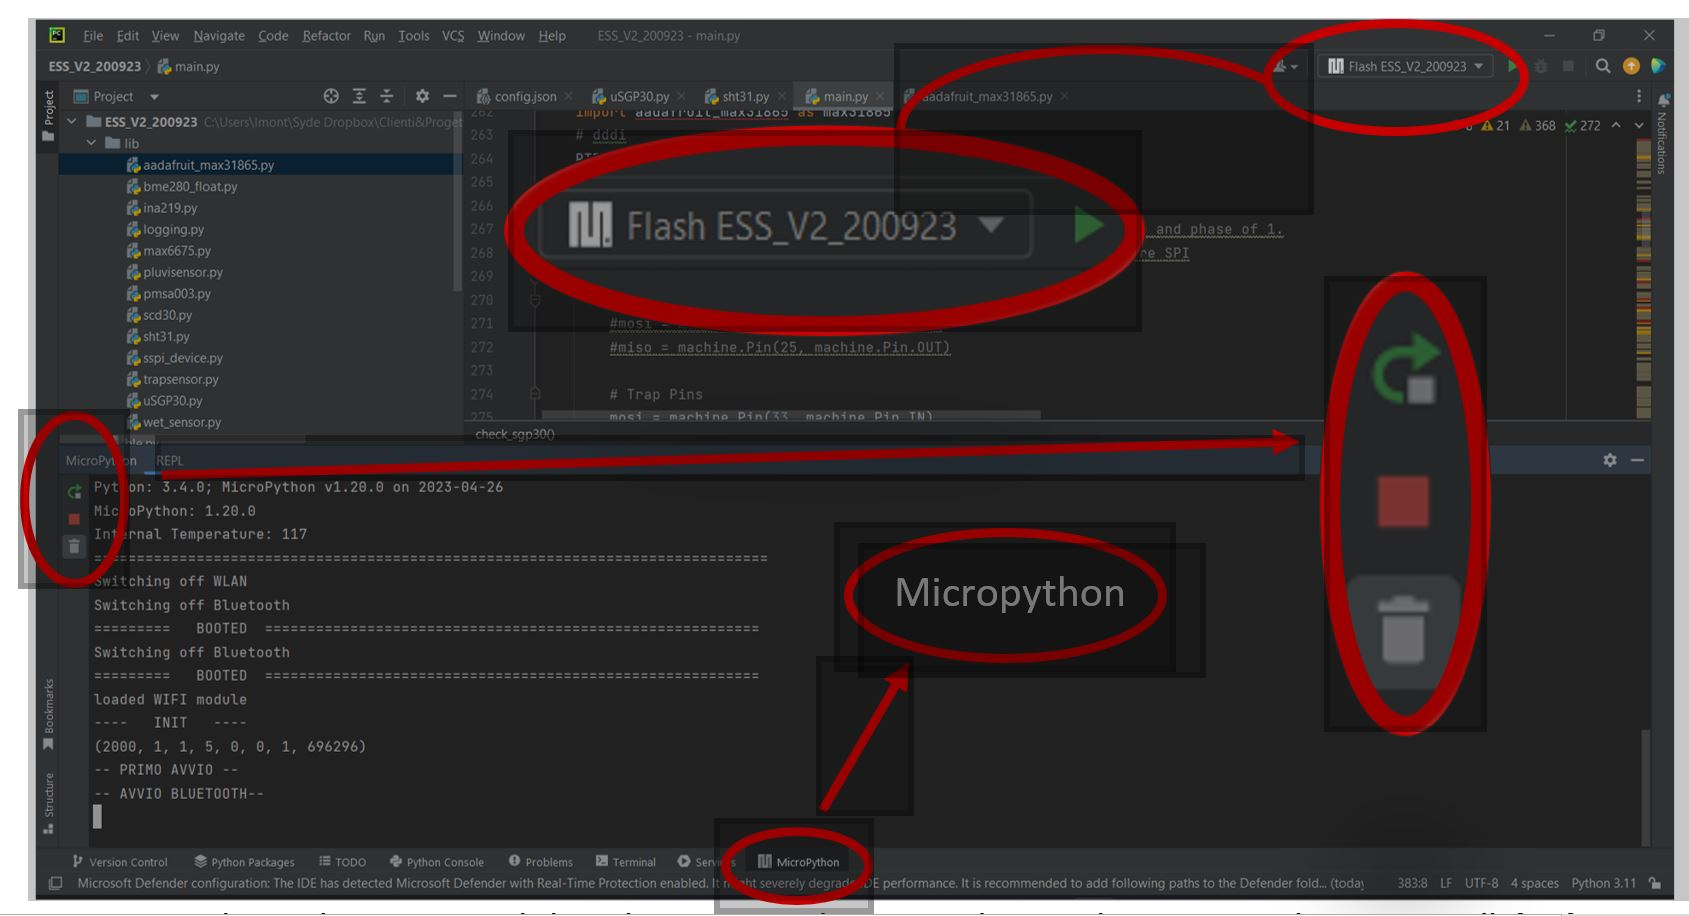
\includegraphics[width=\textwidth]{../../Images/Syde/PyCharmConfig}
    \captionof{figure}{Configuration of PyCharm}
\end{center}

- Switch on the sensor from the button, go to the top right and select \menu{Flash ESS\_V2\_200923} or \menu{Flash\_ESS\_V3\_01} and press on the green triangle next to it. If the operation fails, repeat. To see if the operation is working, just take a look at the device monitor and see that the installation is progressing. If blue links appear, then it has failed: repeat.


\medskip

In the case of wanting to load only one tab (e.g. only config.json after editing), we must first open the tab of interest, select 'Current File' and press Play at the side.


\begin{center}
    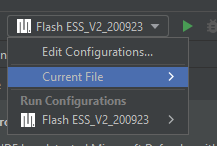
\includegraphics[width=\textwidth]{../../Images/Syde/PyCharmConfig2}
    \captionof{figure}{Flash\_ESS\_V3\_01}
\end{center}


In case of an error, check at  \menu{File > Settings > Project: ESS\_V3\_01 > Python Interpreter} that the Python interpreter is set [Python 3.10 (Acer) or Python 3.11 (MSI)].
In Edit Configurations, check that the Path (=code path) is correctly specified.


\medskip

\begin{center}
    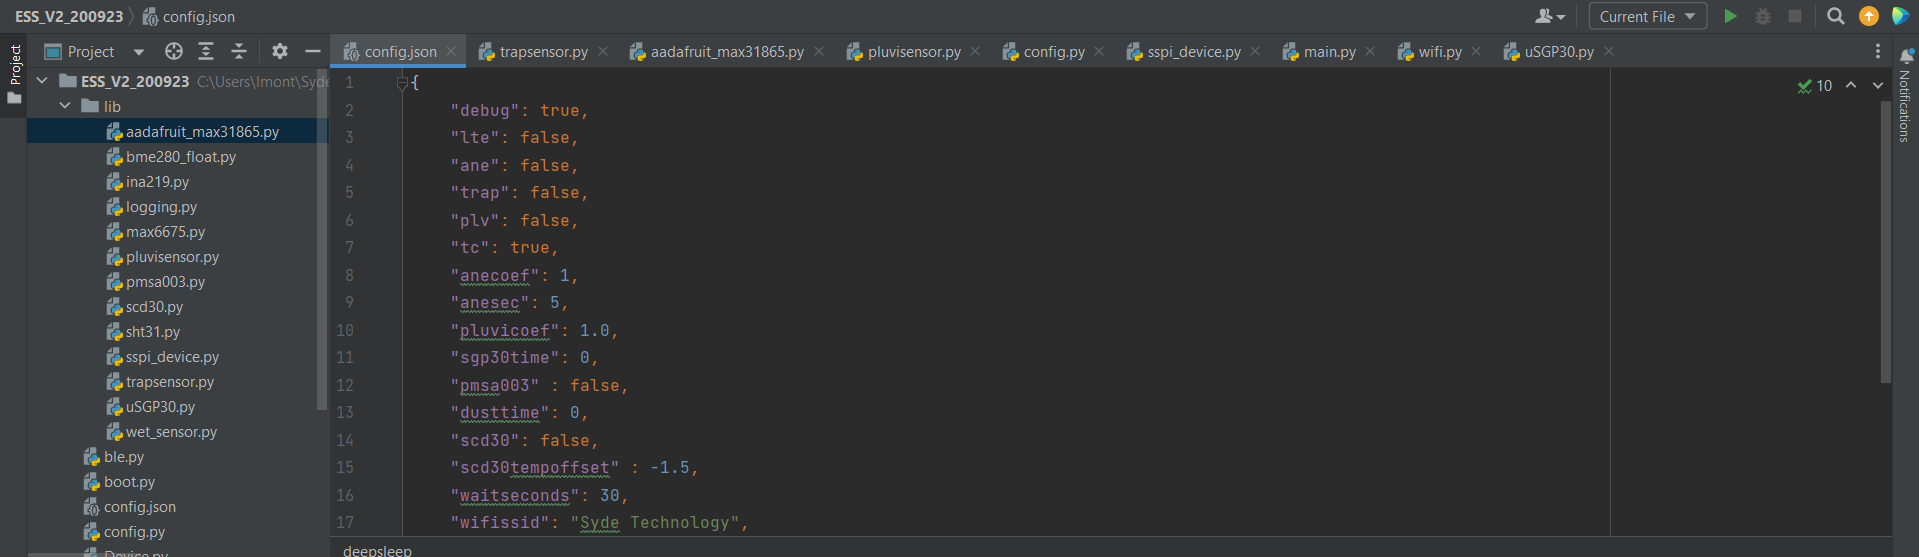
\includegraphics[width=\textwidth]{../../Images/Syde/PyCharmConfig3}
    \captionof{figure}{Flash\_ESS\_V3\_01}
\end{center}


Set \FILE{config.json} before running the sensor for the first time: activate the mounted sensors by substituting \PYTHON{true} for \PYTHON{false} in the corresponding lines, then select \menu{Current File} in the top right bar and press the \menu{Play} button (green triangle).

"deepsleep" must be set to "true".

"waitseconds" must be 200.

"deepsleepseconds" must be 3400 (the sensor transmits every hour).


"debug" can be set to "true" to see the sensor data in detail.


\bigskip

Next, go to the section \menu{MicroPython} (in the bottom bar), press the green arrow on the left and switch the sensor off and on again from the button.

Important: set "false" to debug once the sensor is finished to reduce consumption.

Important: When uploading the firmware, remember to set the correct calibration values for WET, IRR and CO2(indoor sensor) !!!

\section{FW installation on AZ Delivery / Lopy (OLD SENSORS)}

In order to install the FW on an AZ Delivery/LOPY card, it is necessary to use the ACER PC. The first thing to do (one-off on a new card) is to install the FW on EPS 32 by following the guide on the pages above exactly, bearing in mind the COM port the device has taken. This procedure is not to be done for LOPY cards. For these you need to use the "Pycom Firmware Update" program (only to be done if the board is new, placing the lopy over the expansion board and making sure that the orange led next to it is lit).


\begin{center}
    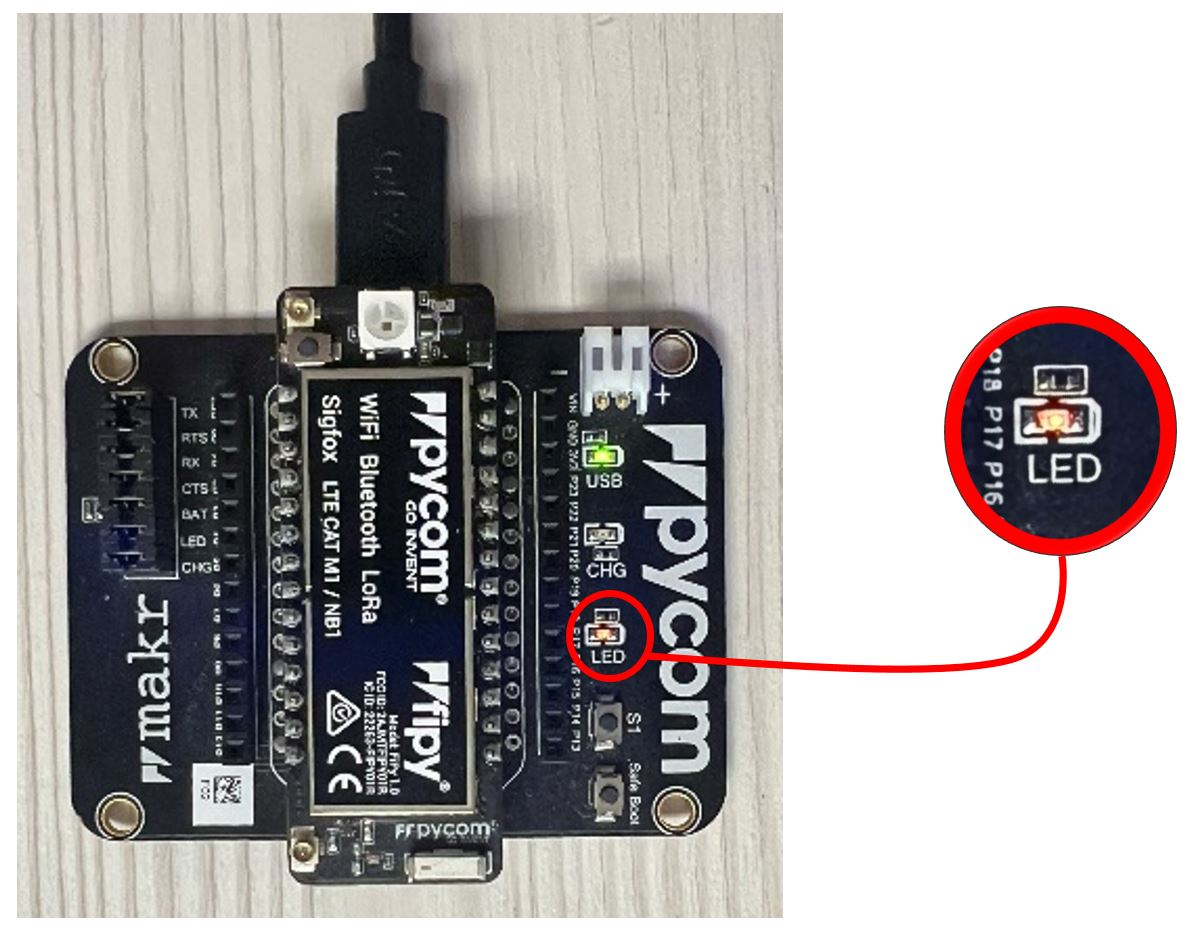
\includegraphics[width=\textwidth]{../../Images/Syde/OldSensor}
    \captionof{figure}{Old Sensor}
\end{center}

After that you can move on to installing the FW on the board, using Visual Studio Code. The difference between AZ and LOPY is that with AZ you have to make the connection manually, whereas with LOPY you can take advantage of the auto-connect function.

\bigskip

AZ: Once Visual Studio Code is open, we must remove the auto-connect setting and set the right port. To do this, simply click on "ALL COMMANDS" at the bottom (1) and select "GLOBAL SETTING" (2)


\begin{center}
    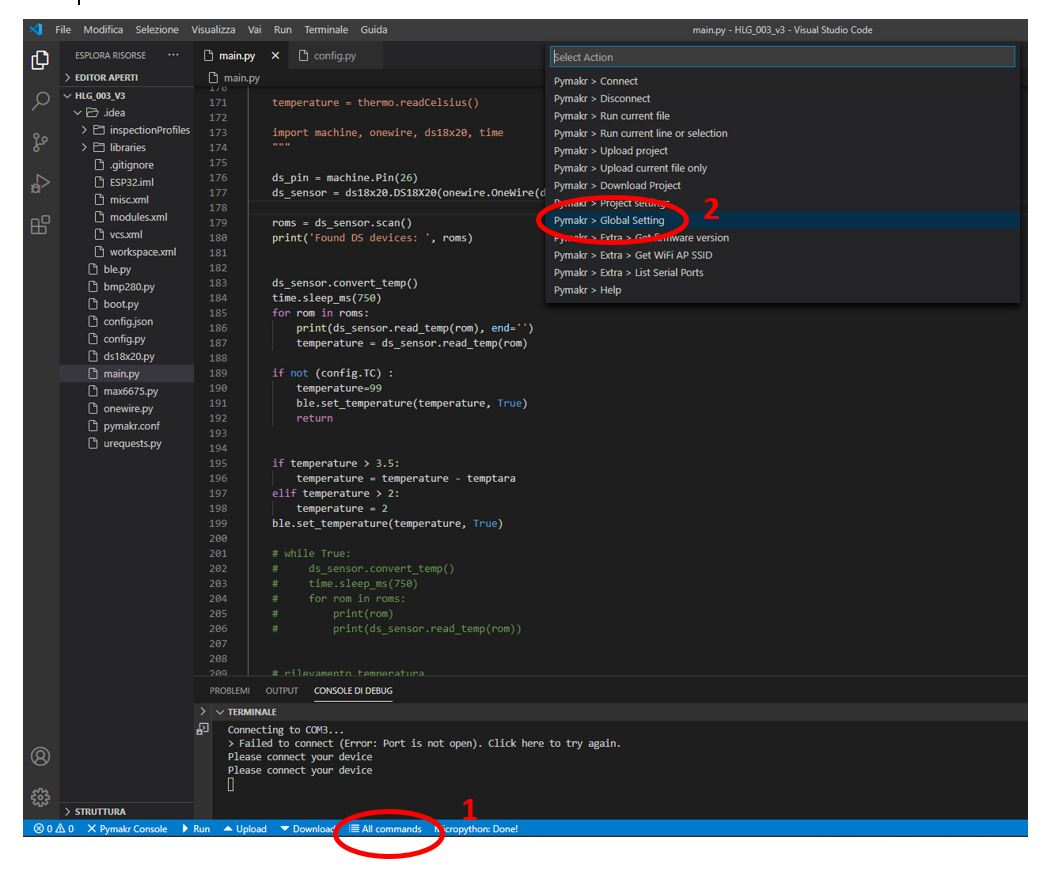
\includegraphics[width=\textwidth]{../../Images/Syde/OldSensorSettings}
    \captionof{figure}{Old Sensor Settings}
\end{center}


We must now enter "COM" (3) and check that ``auto\_connect'' is set to "false"(4). If it is not, simply delete "true" and write "false" and then save, pressing "CTRL+S" and paying attention to the comma, which must remain. Once this is done, it is possible to connect the device.

\begin{center}
    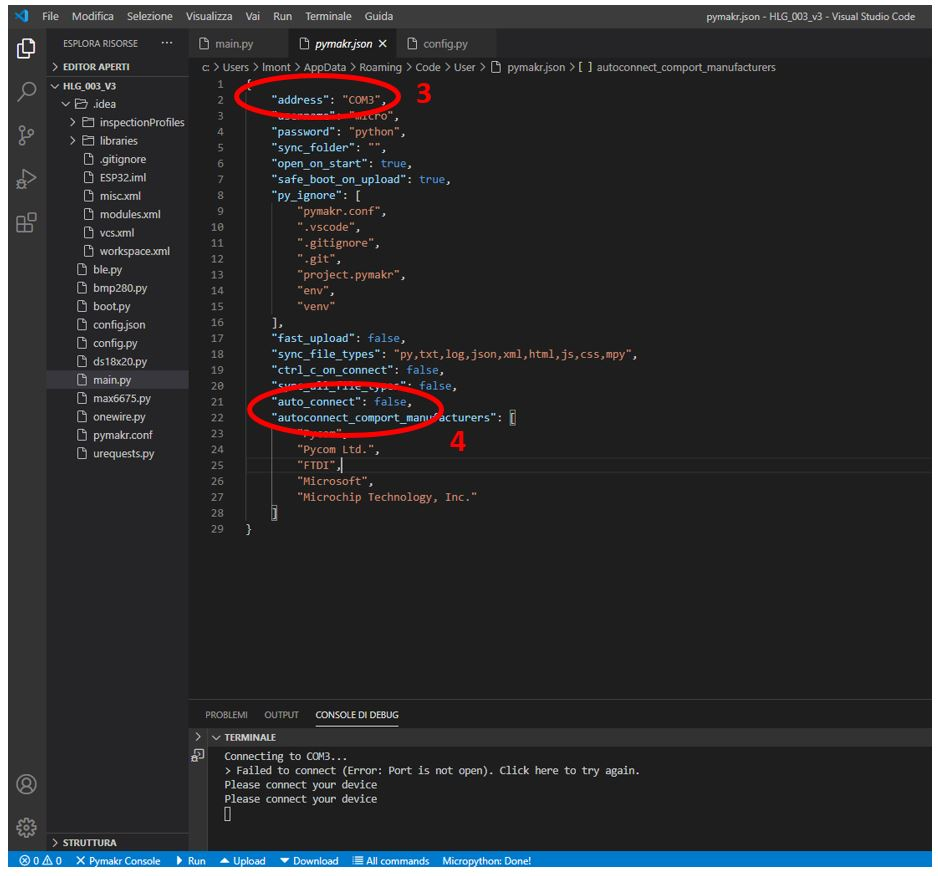
\includegraphics[width=\textwidth]{../../Images/Syde/OldSensorSettings2}
    \captionof{figure}{Old Sensor Settings 2}
\end{center}


To connect a device we have to click again on "ALL COMMANDS" (5) at the bottom and then on "CONNECT" (6). Once the device is connected, we can upload the FW by clicking on ``UPLOAD'' at the bottom (7). All that remains now is to wait for the upload, after which the device will reboot automatically. I still recommend disconnecting and reconnecting the device (steps 5-6)


\begin{center}
    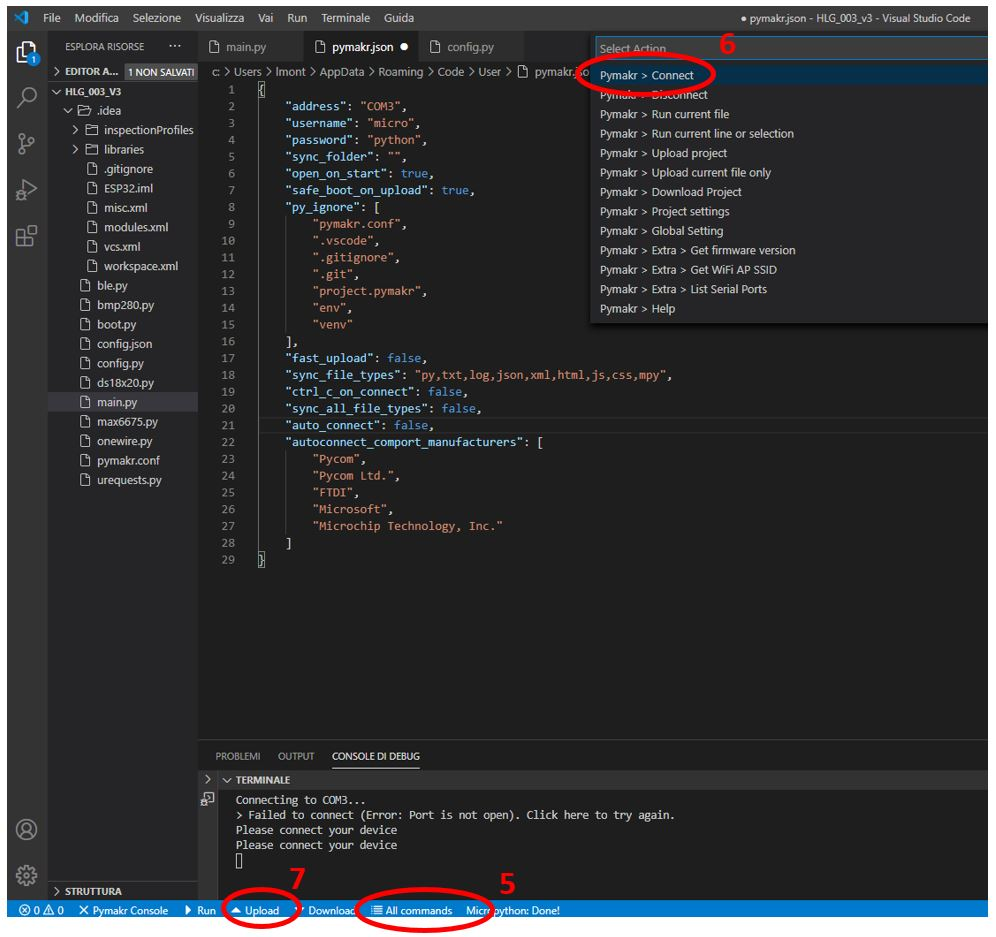
\includegraphics[width=\textwidth]{../../Images/Syde/OldSensorSettings3}
    \captionof{figure}{Old Sensor Settings 3}
\end{center}


LOPY: Once we have placed the lopy on top of the expansion board and verified that the LED is on, we must check that the autoconnect setting is enabled. To do this, simply go to the "global setting" tab and set the autoconnect to "true" if it is set to false. CHECK AZ. GUIDE
Once connected, press "CTRL+C" repeatedly to stop the running programme (visible from the terminal). Once the programme has stopped, press UPLOAD (7) and wait for the process to complete.


\begin{center}
    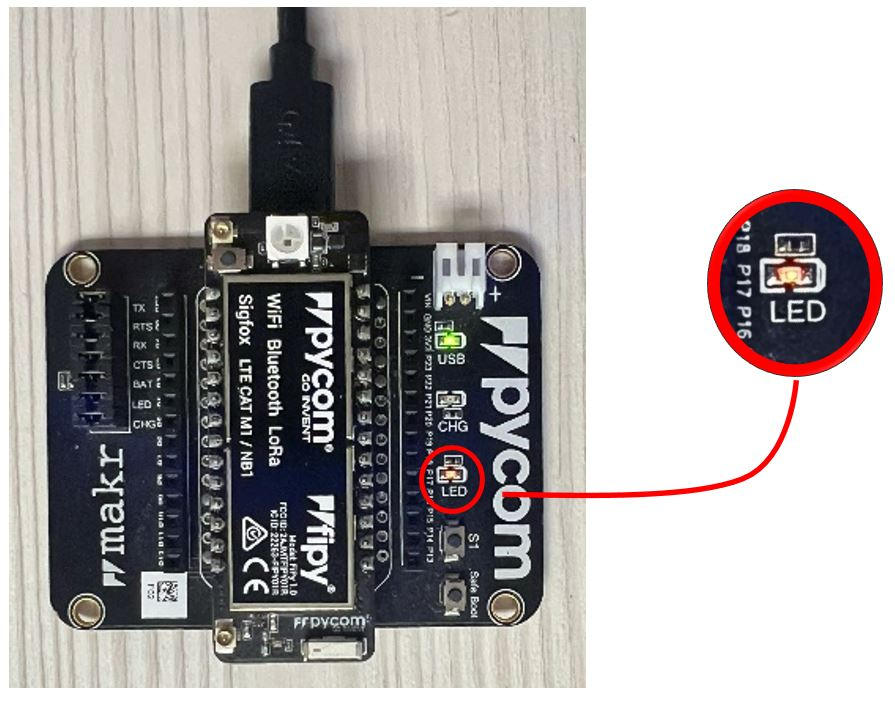
\includegraphics[width=\textwidth]{../../Images/Syde/OldSensor2}
    \captionof{figure}{Old Sensor2}
\end{center}


\section{I2C sensor cable assembly}


\begin{center}
    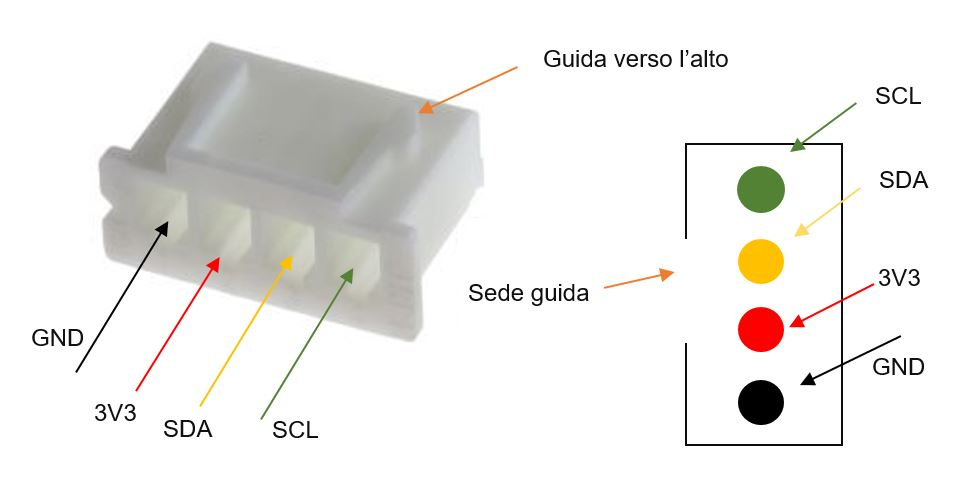
\includegraphics[width=\textwidth]{../../Images/Syde/I2CConnector}
    \captionof{figure}{I2C Connector}
\end{center}

\section{Cable assembly PLV, TRAP, WET}

PLV, TRAP and WET are fitted with black crimped leads, to be soldered to the boards with tin.

\begin{center}
    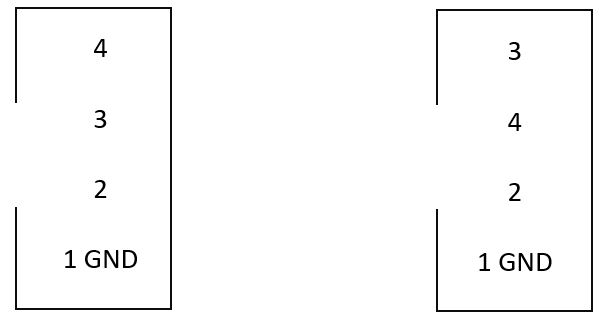
\includegraphics[width=\textwidth]{../../Images/Syde/I2CConnector2}
    \captionof{figure}{I2C Connector}
\end{center}

\section{Board details}

\begin{center}
    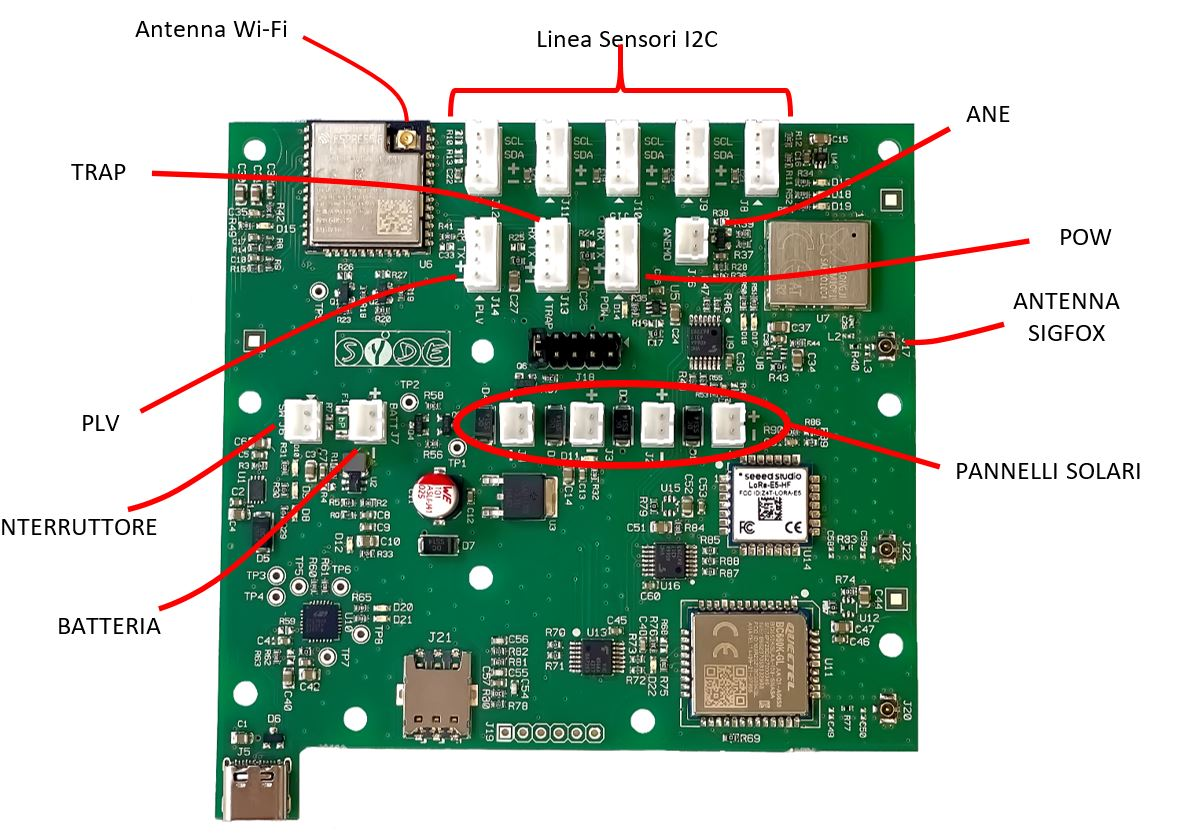
\includegraphics[width=\textwidth]{../../Images/Syde/BoardDetails}
    \captionof{figure}{I2C Connector}
\end{center}

NB: spray tropicant on each board and sensor before mounting them, covering the white connectors and antenna connectors with tape first.

Note: If the anemometer does not work, the sensor is too high, too low or not working (check with multimeter).


\section{Special Case: PT100 + MAX31865}

Jumper to be soldered as in photo.

\begin{center}
    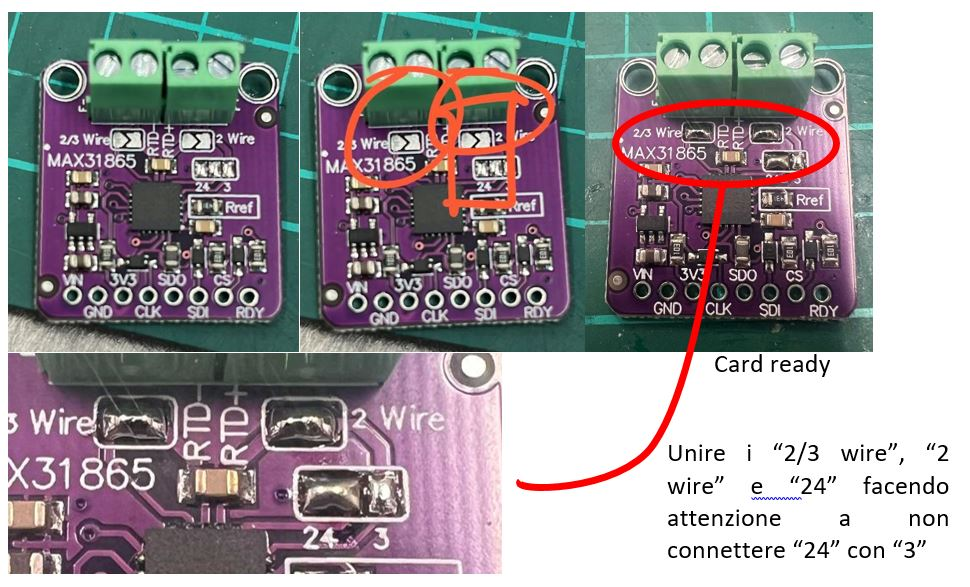
\includegraphics[width=\textwidth]{../../Images/Syde/PT100}
    \captionof{figure}{I2C Connector}
\end{center}



This sensor, in the current version of the board, does not have an ad hoc (6-pin) connector, so for the time being 3 different 4-position JST connectors are required, connected in the following way:

\begin{center}
    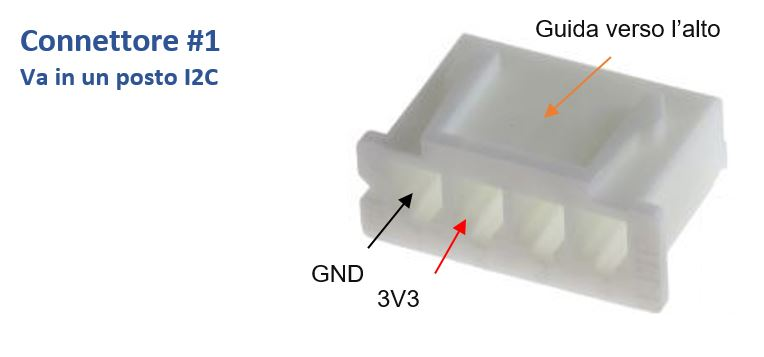
\includegraphics[width=\textwidth]{../../Images/Syde/PT100Connector}
    \captionof{figure}{I2C Connector}
\end{center}


% Seite 16

Connector \#2

Goes in the POW slot

\begin{center}
    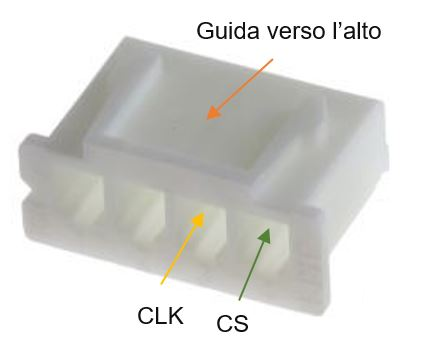
\includegraphics[width=\textwidth]{../../Images/Syde/Connector2}
    \captionof{figure}{Connector}
\end{center}


Connector \#3

Goes in the PLV or TRAP 

\begin{center}
    \includegraphics[width=\textwidth]{../../Images/Syde/Connector3}
    \captionof{figure}{Connector}
\end{center}


NB: The position of this connector varies from sensor to sensor and the correct connection must be set on the FW (in main.py) each time, otherwise the temperature read out will be a value completely out of scale!!! (see next page).

\begin{center}
    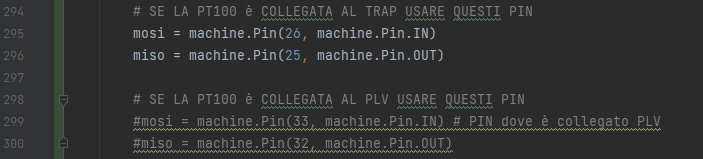
\includegraphics[width=\textwidth]{../../Images/Syde/Connector23}
    \captionof{figure}{Connector}
\end{center}

In the case of the screen, the MAX31865 is connected in the TRAP slot.


\section{Trap}

\begin{center}
    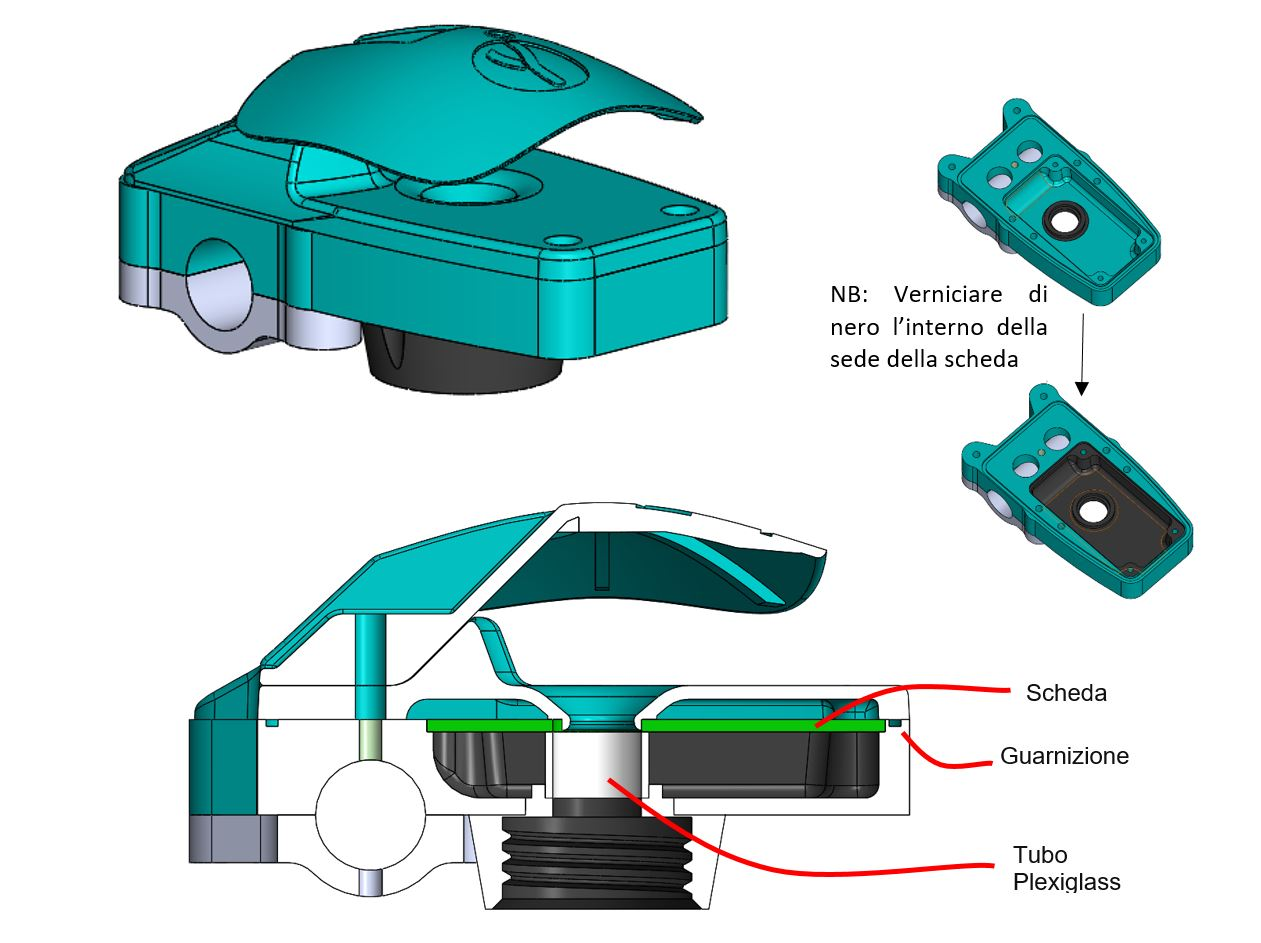
\includegraphics[width=\textwidth]{../../Images/Syde/Trap}
    \captionof{figure}{Trap}
\end{center}



exe file to test the TRAP: \URL{C:/Users/lmont/Syde Dropbox/Clients&Projects/Syde/Models/Compolab/BRD_SENS_TRAP/wetransfer_results_trap_sensor_updated_2022-06-17-pdf_2022-06-17_1621/SYDETrapMonitor}

Connect the TRAP to the PC via the appropriate cable, see the port to which the TRAP is connected (e.g. COM10), open the exe file, select the port and click on Connect, select Trigger


\menu{Calib > Send}, Set \menu{Autocalib > Send}, \menu{Get Status > Send} (Autocalibration must be true), test the TRAP and click Send again.

\section{WET}

\begin{center}
    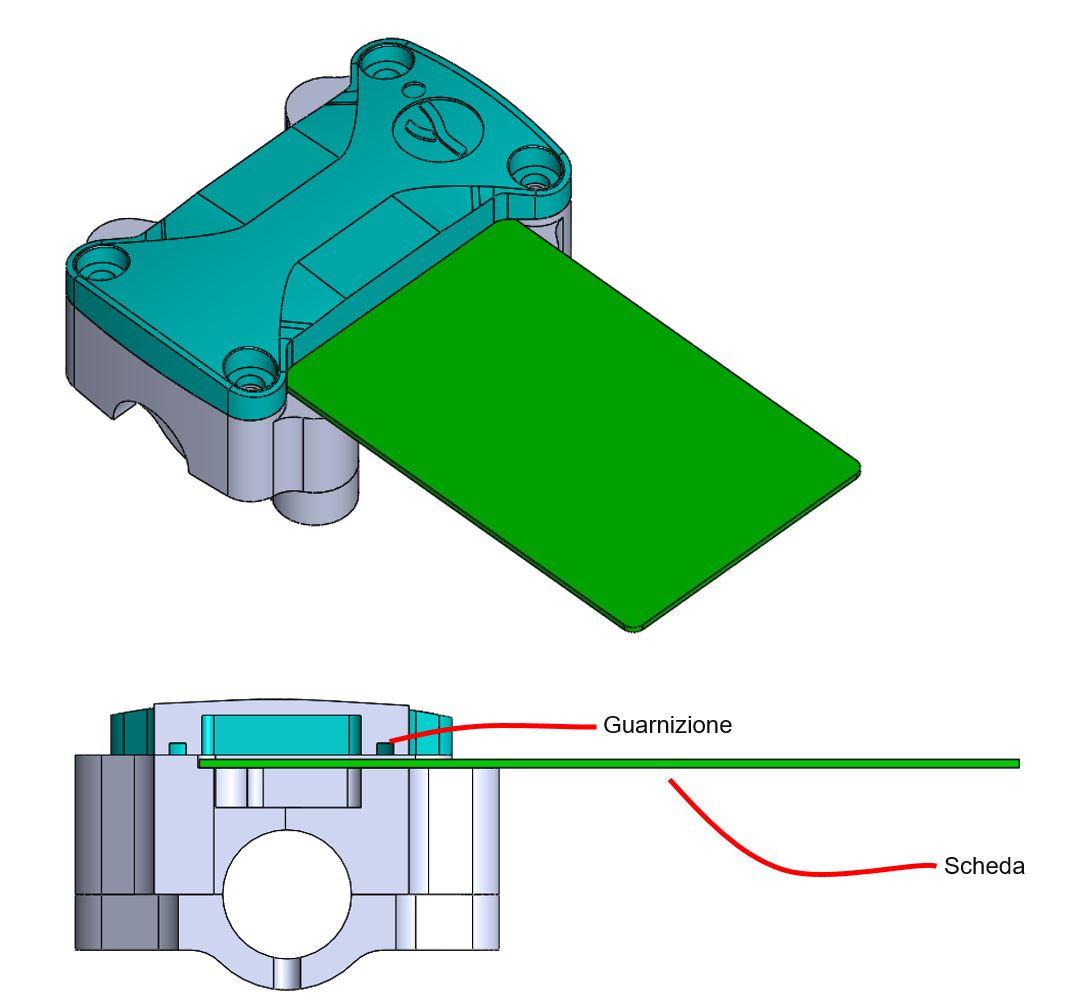
\includegraphics[width=\textwidth]{../../Images/Syde/WET}
    \captionof{figure}{WET}
\end{center}

\section{PLV}


\begin{center}
    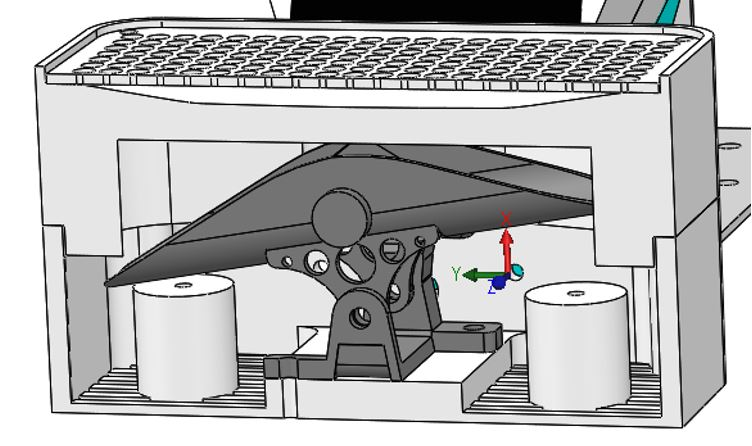
\includegraphics[width=\textwidth]{../../Images/Syde/PLV}
    \captionof{figure}{PLV}
\end{center}

Note: After soldering the leads to the board, put hot glue on the board pins to insulate them.

BOARD INSTALLATION

- Visual Studio Code with STM32-for-VSCODE plugin

\section{PLV CARD INSTALLATION}


\begin{center}
    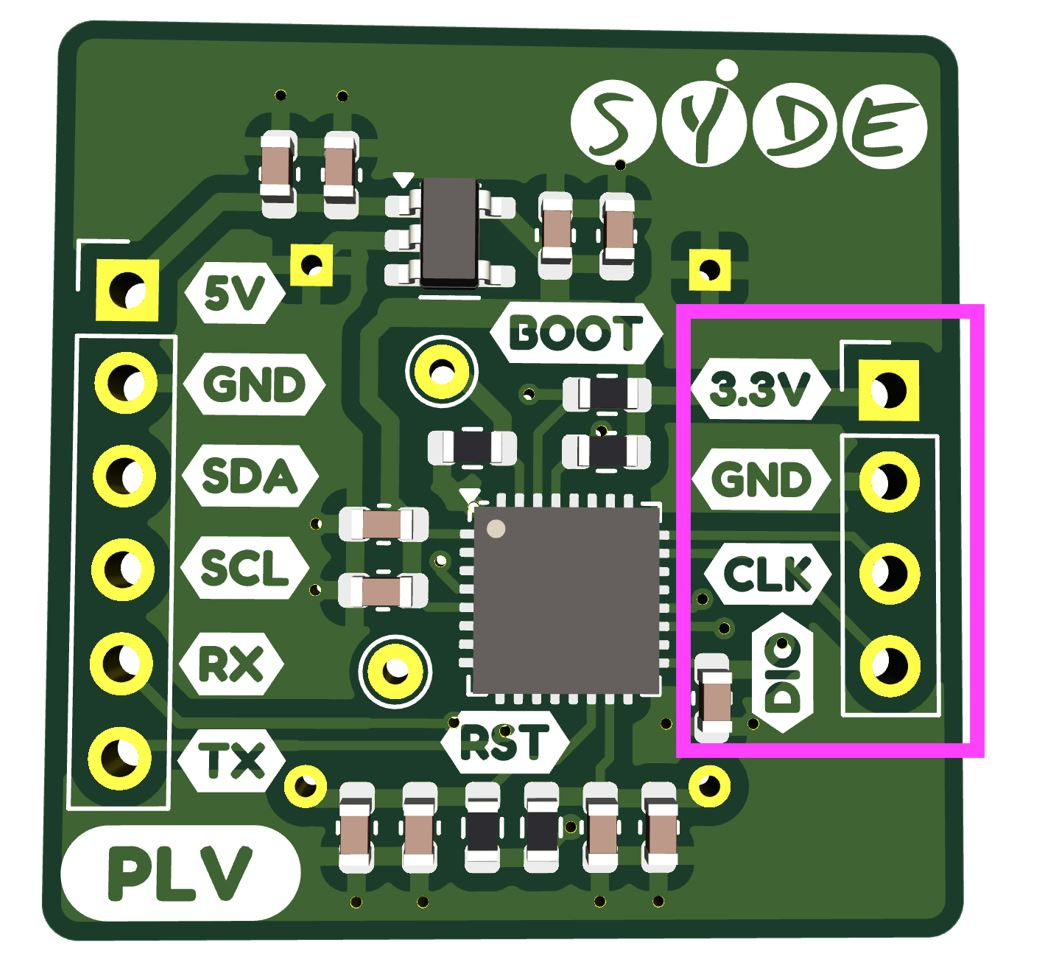
\includegraphics[width=\textwidth]{../../Images/Syde/PLVBoard}
    \captionof{figure}{PLV Board}
\end{center}

The programming PINs are 4 on the right, two are the power supply (3.3V and GND) the others are CLK and DIO, clock and data. These 4 pins only need to be connected when flashing the firmware, after that they are of no use. So you can also use flying jumpers if you wish, the important thing is that they make contact.

To programme these devices, you need the ST-LINK V2 programmer, which must be connected in the correct way. There should be a ready-made wiring harness to do this, so just connect it the right way, double-checking all 4 PINs.

\section{SOFTWARE}

The PLV software is available on SYDE's GitHub repo, username syde2024.

\begin{center}
    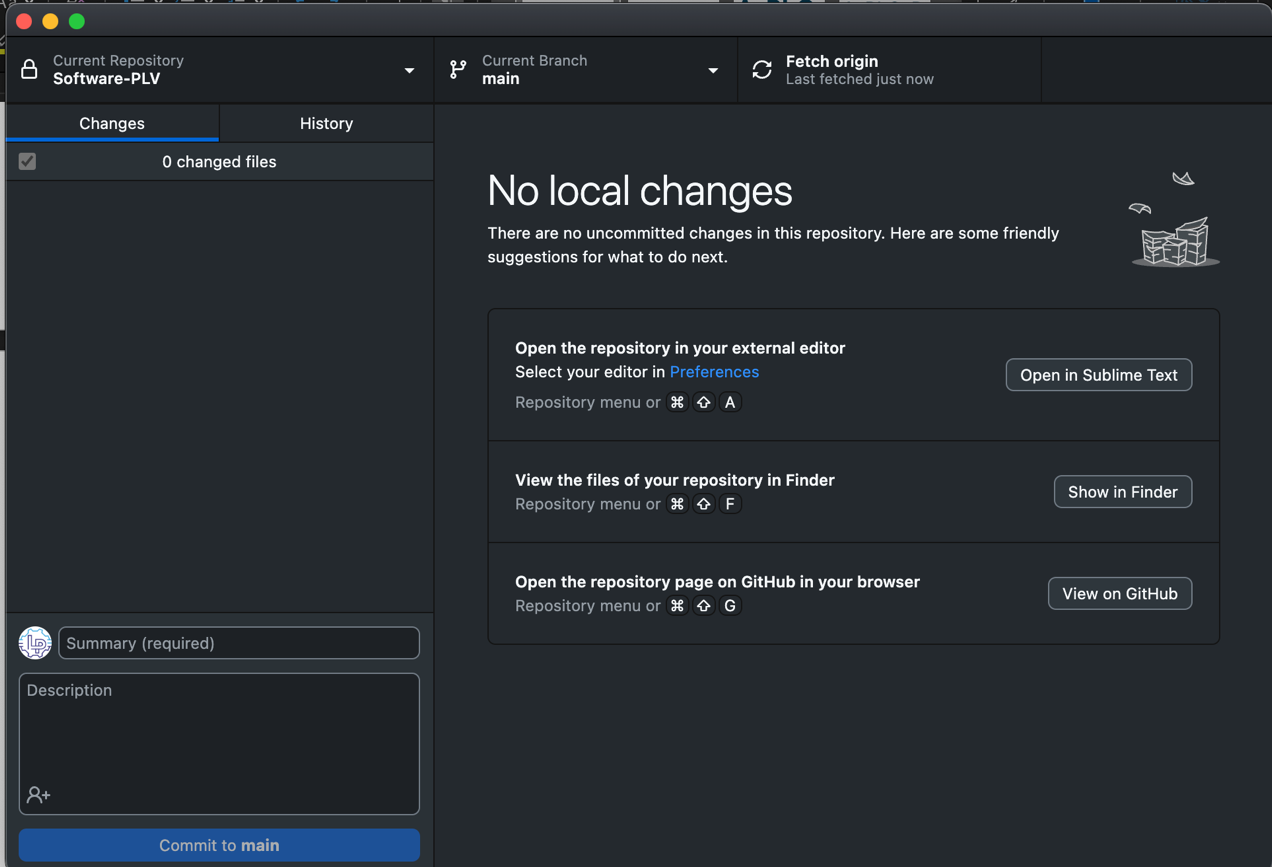
\includegraphics[width=\textwidth]{../../Images/Syde/SydeGithub}
    \captionof{figure}{Syde's Github}
\end{center}

We use GitHub Desktop to access and keep the firmware synchronised at all times.

If we see that when we click on fetch origin there is no update, it means that we are at the latest version. Or that someone else has not uploaded the update.

We now open Visual Studio Code and go to the folder in which our project is located.
Remember that we are using the STM32 for VSCode plugin.

\begin{center}
    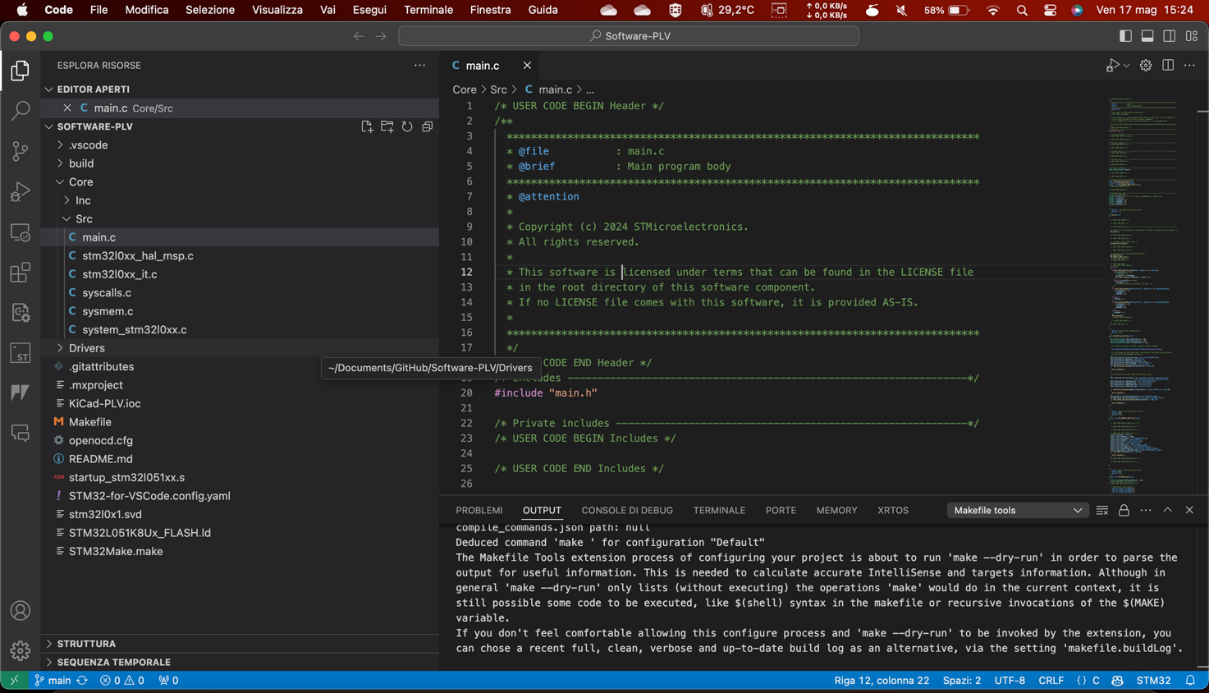
\includegraphics[width=\textwidth]{../../Images/Syde/GitHubCode}
    \captionof{figure}{Syde's Github Code}
\end{center}

% Seite 24

Once the folder is open, click on the plugin

\begin{center}
    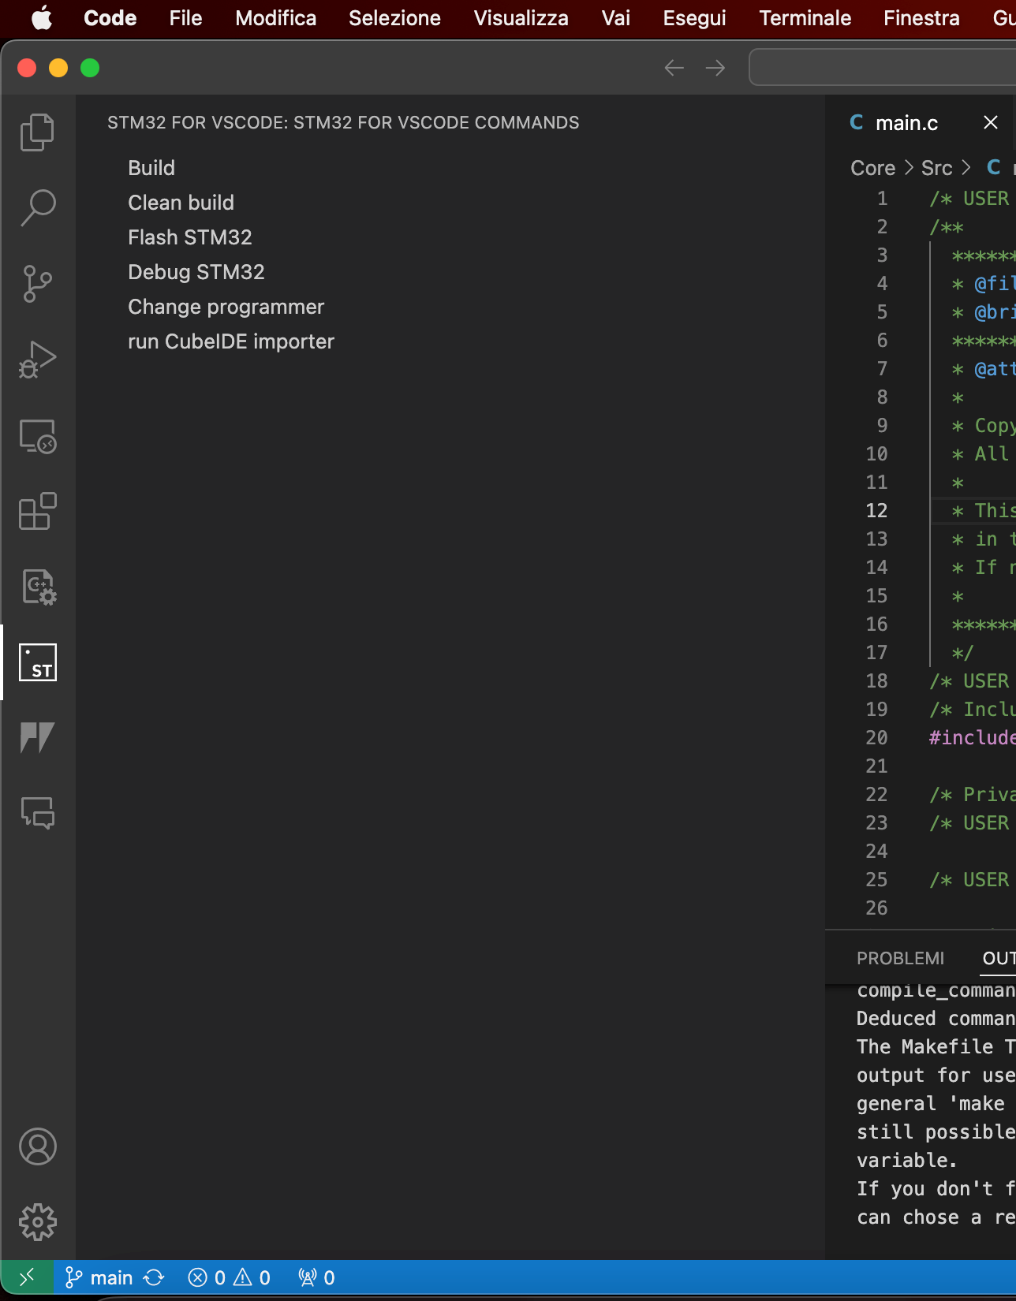
\includegraphics[width=\textwidth]{../../Images/Syde/Plugin}
    \captionof{figure}{Plugin}
\end{center}


STM32 and click on Clean Build to compile the programme. Once it is finished we can click on Flash STM32 to load the programme on the rain gauge. Once loaded we unplug everything and we are done.


For the wiring on the ESS we use the other connector, but in this case we solder 4 wires: two are the power supply (5V and GND) the others are TX and RX, which are the serial data. Remember also to solder the REED sensors which are at the back.


\begin{center}
    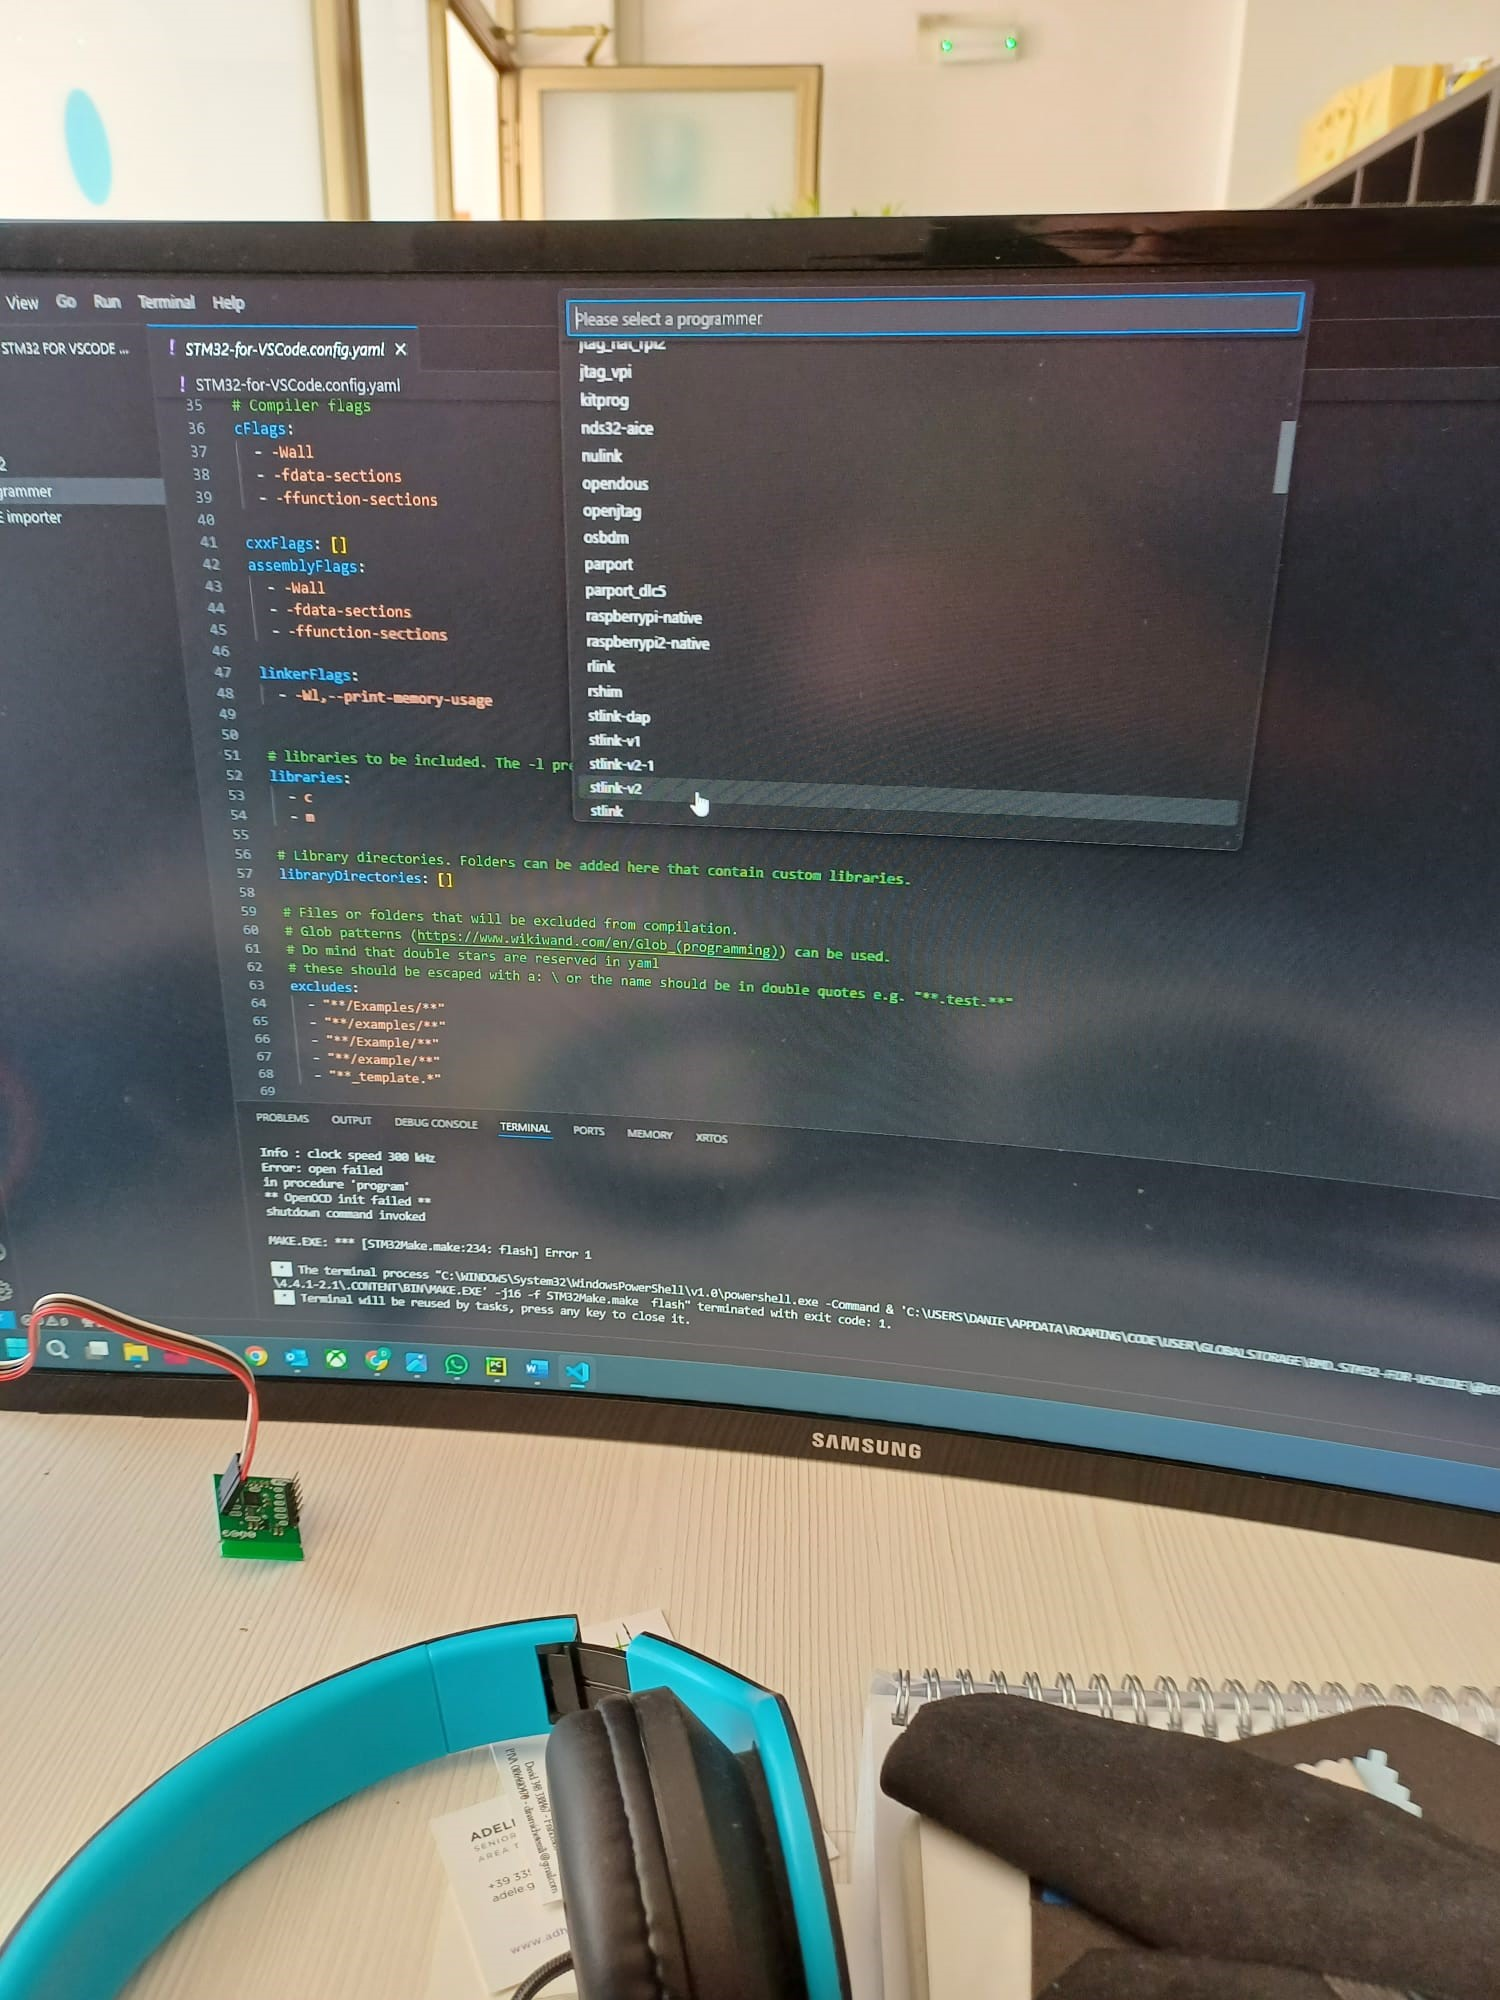
\includegraphics[width=\textwidth]{../../Images/Syde/Plugin2}
    \captionof{figure}{Plugin 2 } 
\end{center}


\begin{center}
    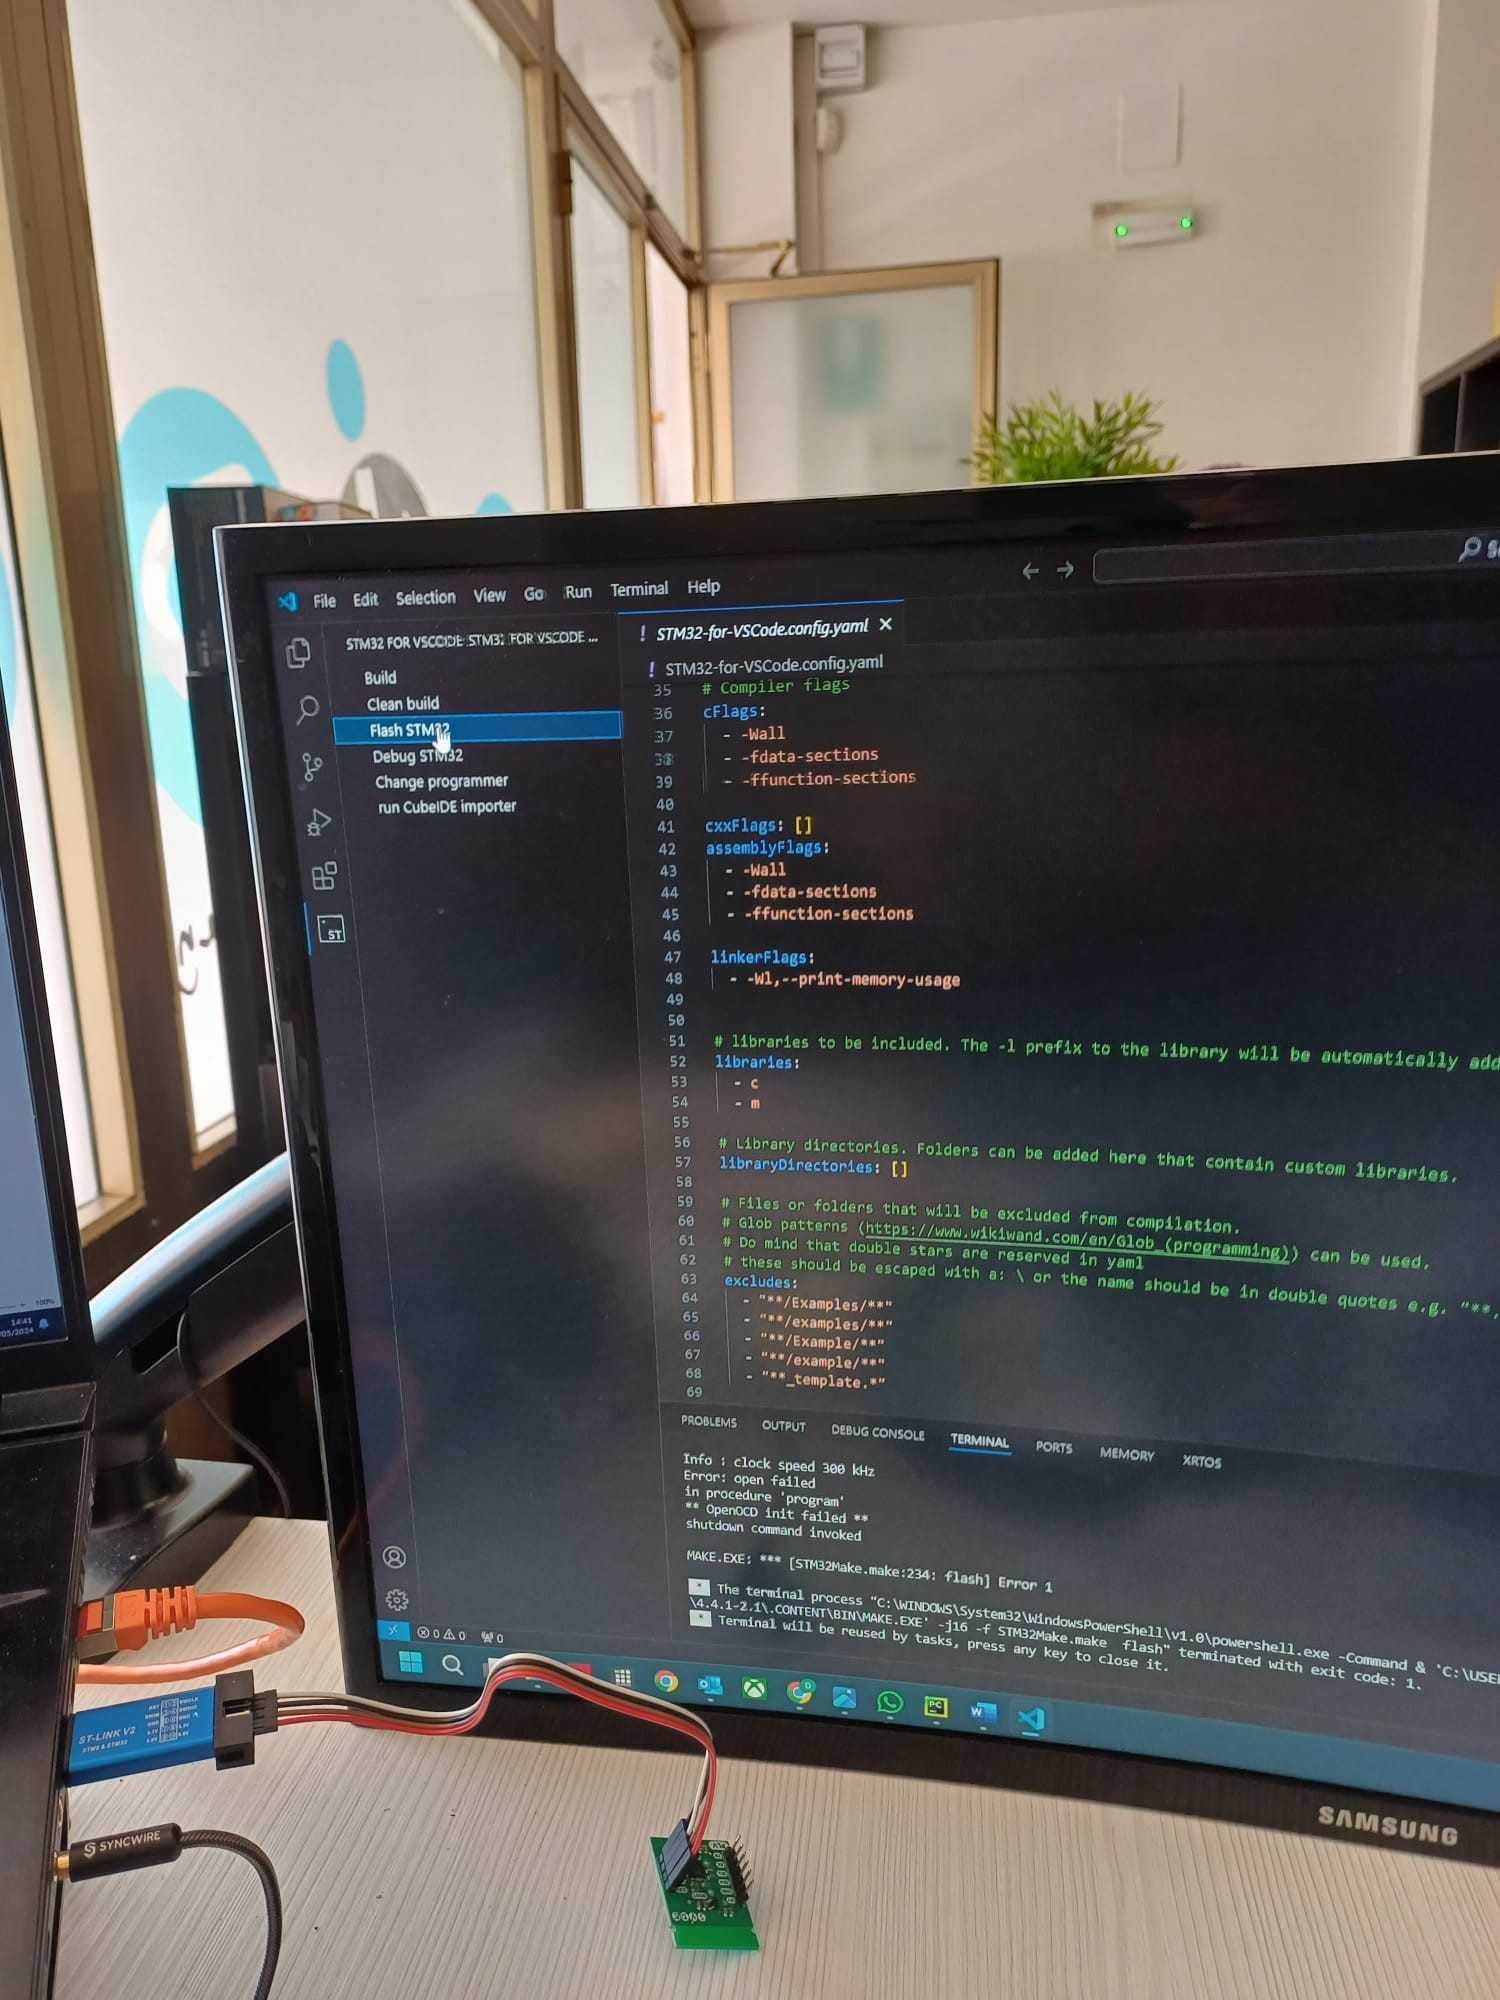
\includegraphics[width=\textwidth]{../../Images/Syde/Plugin3}
    \captionof{figure}{Plugin 3} 
\end{center}


Before flashing the card with the stick, check whether the drivers are installed by going to Device Manager. If they are not installed, right-click and select Update Drivers; install the drivers in the Dropbox, under \menu{Equipment and softwar > STLINK}.


\section{Sensor interior}

\begin{center}
    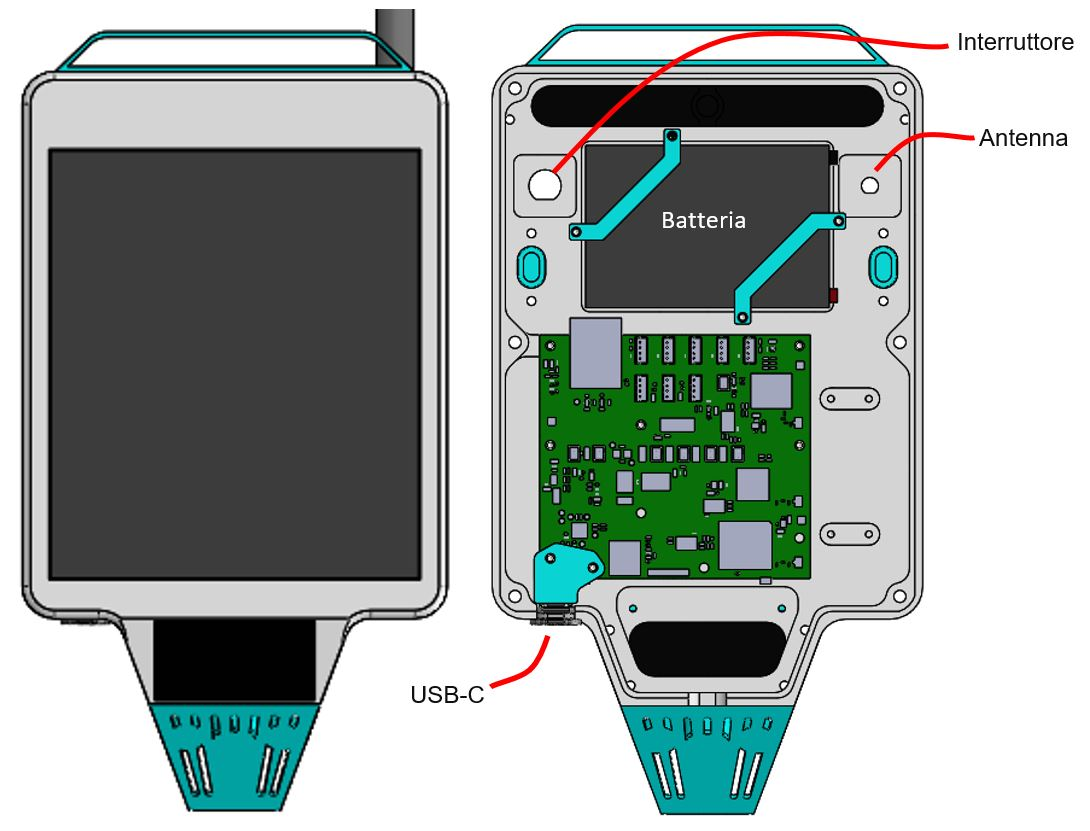
\includegraphics[width=\textwidth]{../../Images/Syde/Interna}
    \captionof{figure}{Interna} 
\end{center}


Note: remember to put the anti-insect net on the top and bottom caps of the base, to be cut with the appropriate cardboard shapes.
\section{Sensor calibration}


\begin{itemize}
    \item  WET (see Excel file): in \FILE{config.py}, set dry value, wet value and difference

\begin{center}
    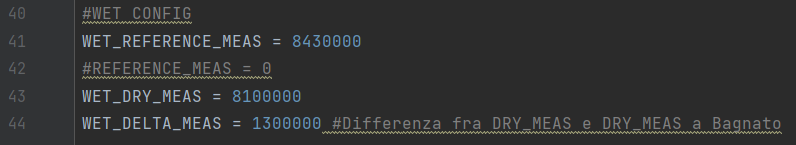
\includegraphics[width=\textwidth]{../../Images/Syde/WETCalibration}
    \captionof{figure}{WETCalibration} 
\end{center}

In \FILE{config.json}, set 'debug' to 'true' to display the values below.

\PYTHON{WET\_REFERENCE\_MEAS} = reference circuit reading, this is the second number (CHANNEL 1) that appears in debug measurements; it must be averaged over the different readings

\begin{center}
    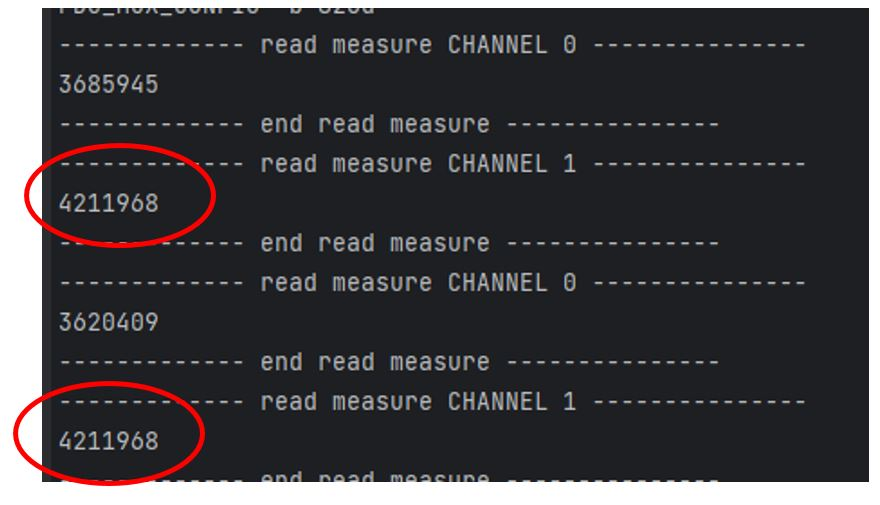
\includegraphics[width=\textwidth]{../../Images/Syde/WETCalibration2}
    \captionof{figure}{WETCalibration} 
\end{center}

 \PYTHON{WET\_DRY\_MEAS} = dry sensor reading, it is the first number (CHANNEL 0) appearing in debug measurements; it must be averaged over the different measurements
 
      The wet measurement is to be repeated.

\begin{center}
    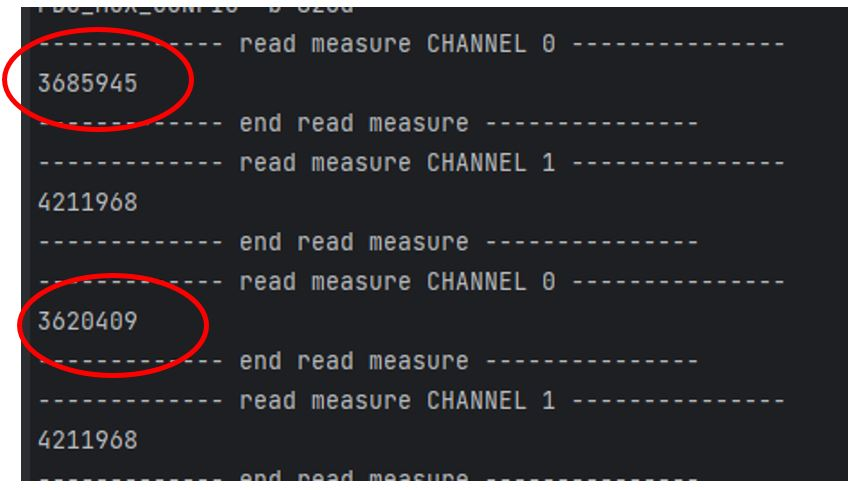
\includegraphics[width=\textwidth]{../../Images/Syde/WETCalibration3}
    \captionof{figure}{WETCalibration} 
\end{center}
 
 \PYTHON{WET\_DELTA\_MEAS} = difference between dry and wet sensor reading, difference of averages.
 
 USE EXCEL FILE to calculate the values to be set.
 
 \item  IRR: in \FILE{config.json}, set the variable "calibrationIRR" equal to the correction coefficient evaluated by experimental test, equal to (device reading)/(sensor reading)
 \item PLV: adjust both grains so that the bascule falls with 0.5 mm of water (if the grains are higher, the bascule falls sooner)  with a syringe 27 mL of water and count 10 touches of the bascule (calculation: sup plv (5355 $mm^2$) x 0.5 = 2.678 mL)
 
 \item CO2 (SCD30) (for internal use): enter a numerical value in the config.json file under 'scd30forcerecal'. Once the device has been restarted, recalibration to the value will be forced, after which this value will be set to zero and will no longer be recalibrated.
 
 Notes:
   \begin{itemize}
       \item in \FILE{config.py} there is a value that changes the temperature (temperature = temperature + config.SCD30\_TEMP\_OFFSET), which can be set in \FILE{config.json}. This was needed because the old Lopys had the processor close to the sensor and heated it up by 1 to 1.5 degrees. To be set according to context.
  \item in \FILE{main.py} there is a procedure whereby the sensor result is an average of the last valid readings taken, which is present because in old boards there were connection problems.
   \end{itemize}
 
\end{itemize}

 \section{Sigfox}
 
     This is the network on which the sensors communicate.
     
     Active contracts are currently provided by EIT service. The contact persons are:
     
     \bigskip
     
     \begin{itemize}
         \item for the technical part Ferro Luigi (Luigi.Ferro@Eitowers.it)
         \item Ei Towers ServiziCommerciali-EIT@eitowers.it for the commercial part
     \end{itemize}

     And we have to send an email to them every time we decide to activate new devices.
     
     \bigskip
     
     To work, a Sigfox device needs 2 things:
     
     \begin{itemize}
         \item \textbf{Device activation:} to activate a new device we have to retrieve the necessary codes from our device, which are:
     \begin{itemize}
       \item  SIGFOX ID
       \item SIGFOX PAC
     \end{itemize}

     These have to be communicated to Mr Ferro asking for the activation of the device(s) in the same way as before. Doing this will activate the devices, which will automatically go into the same group and device type as those already created. The contracts activated so far have (per day)

     \begin{itemize}
       \item  140 Uplinks (the messages we send)
       \item  4 Downlinks
     \end{itemize}
 
     This is the end of Mr Ferro's part. He generally activates them within the day or a maximum of 2 days.
       \item  \textbf{Availability of the communication token:} this is generally the longest part and is in the hands of EIT's commercial services. They have to send us the usual offer and we have to send it back signed.
     \end{itemize}
     
\section{Sigfox PAC and Sigfox ID}
    
    Once a new board has been activated (FW installation procedure on ESP32) we must first install the FW taking care to set the "debug" option in the config.json file to "true". Set to true, we can upload the FW following the "FW installation on ESS board" guide.
    
\begin{center}
    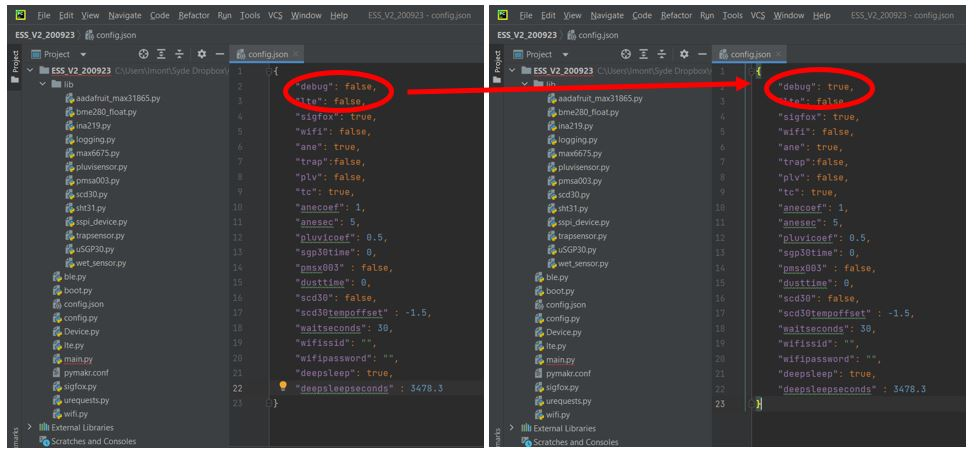
\includegraphics[width=\textwidth]{../../Images/Syde/Sigfox}
    \captionof{figure}{Sigfox} 
\end{center}
         
         
Once the upload is complete, switch the sensor/board off and on again, keeping it connected to the PC so that you can see in real time what the board is doing. The necessary codes will be displayed automatically. These must then be communicated to EIT for activation. The Sigfox ID is the one we commonly see in our sensors, the other is a code they need.

\section{Sigfox backend}
    
    Once these steps have been completed (including the activation of both the device and the contract) we can move to the Sigfox backend in order to assign the new contract to the device. By connecting and authenticating to the following link
    
    \URL{https://backend.sigfox.com/auth/login}
    
    We need to go into the "Device Type" section and click on the group "ESS\_R01".
    
\begin{center}
    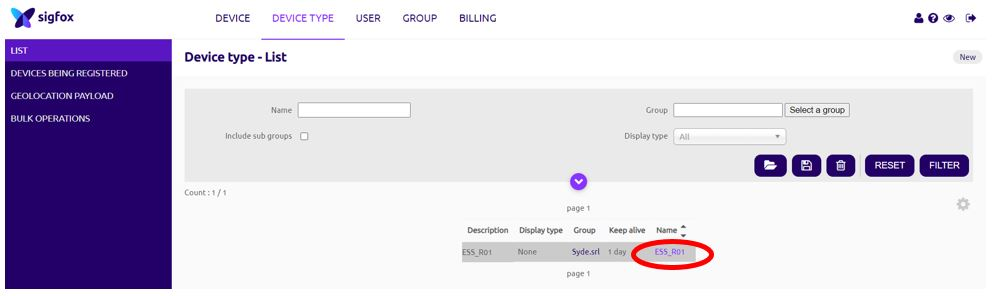
\includegraphics[width=\textwidth]{../../Images/Syde/SigfoxBackend01}
    \captionof{figure}{Sigfox Backend} 
\end{center}
    
    
    
    Poi clicchiamo sul tasto “edit”
             
    
\begin{center}
    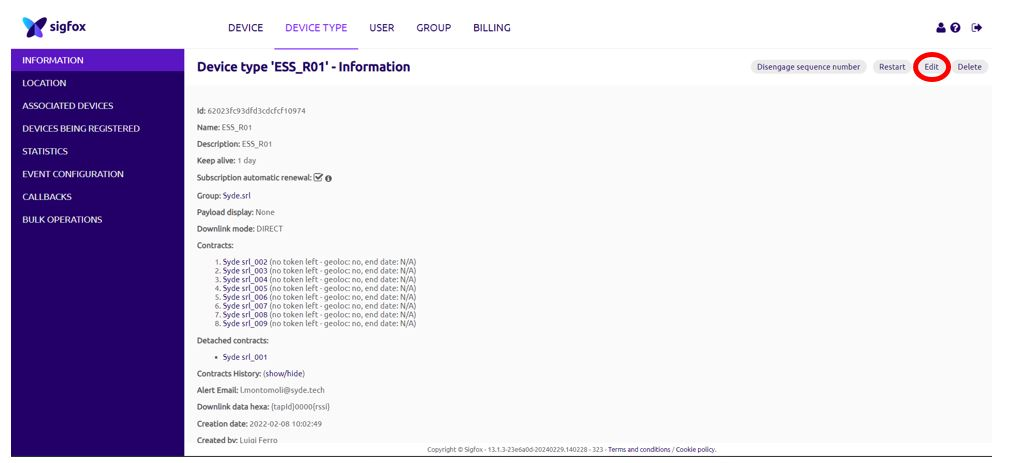
\includegraphics[width=\textwidth]{../../Images/Syde/SigfoxBackend02}
    \captionof{figure}{Sigfox Backend} 
\end{center}


Once on the edit page we must click in the area where all contracts are listed, a drop-down menu will open where new contracts will be shown, we can then enter the new one. Then press OK at the bottom of the page.
NB: Do NOT enter the contract "Syde srl\_001". This is the first contract made and has no active tokens


\begin{center}
    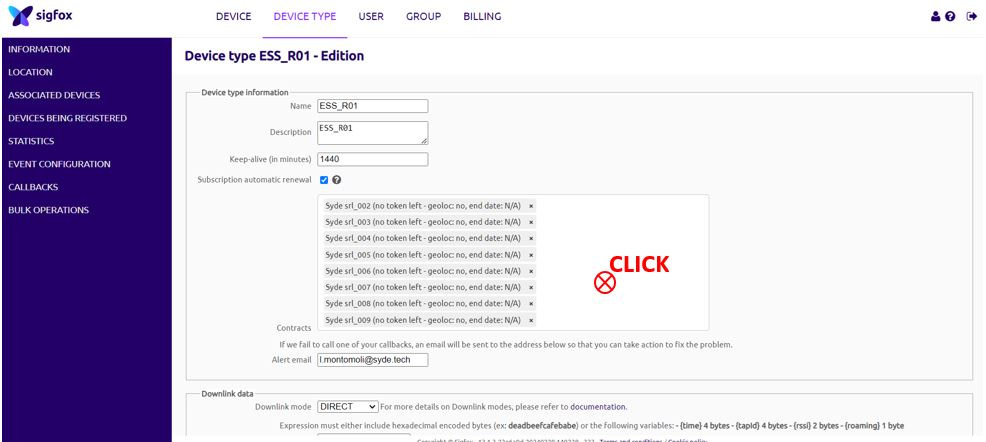
\includegraphics[width=\textwidth]{../../Images/Syde/SigfoxBackend03}
    \captionof{figure}{Sigfox Backend} 
\end{center}

Now that the new contract is entered, we go to the 'device' section and click on the ID of the device we want to activate.

\begin{center}
    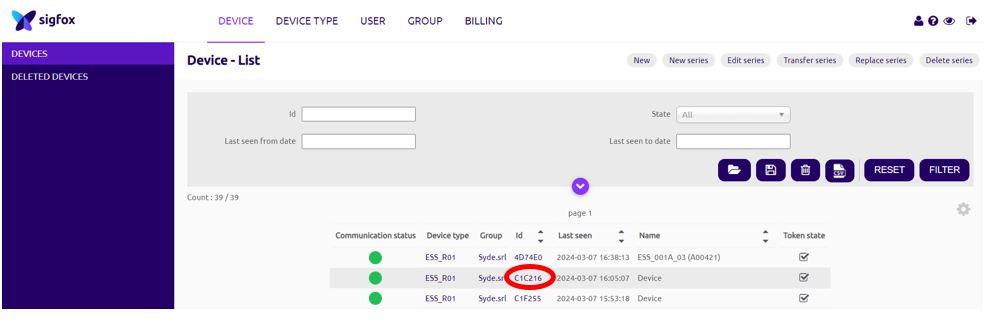
\includegraphics[width=\textwidth]{../../Images/Syde/SigfoxBackend04}
    \captionof{figure}{Sigfox Backend} 
\end{center}

Once connected to the sensor page, we must first suspend and then reactivate the sensor again by clicking on the corresponding buttons.

\begin{center}
    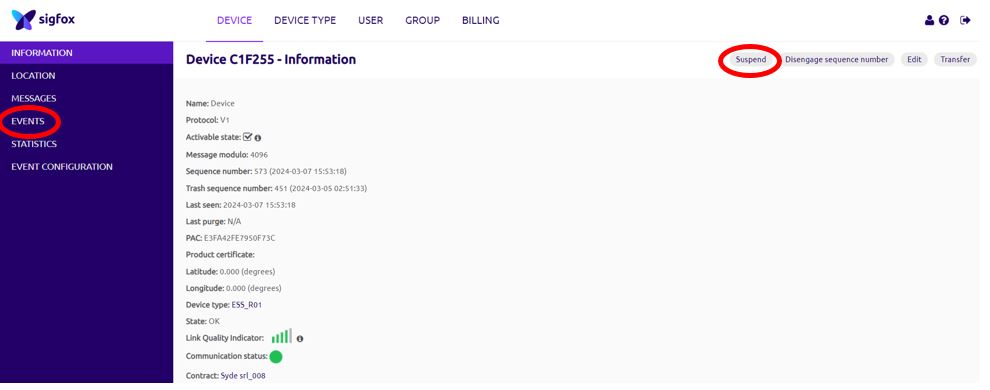
\includegraphics[width=\textwidth]{../../Images/Syde/SigfoxBackend05}
    \captionof{figure}{Sigfox Backend} 
\end{center}

This operation would not be necessary, but it is worth doing. We can now turn on the sensor and have it transmitted. We will see that the first paid message will appear in the 'Events' section and the sensor will also automatically appear in the cloud platform.

NB: to transmit, the antenna must be screwed tightly to the sensor.


\section{Renaming the sensor from app/site}

In the app or on the website, go to \menu{Devices > New devices}, enter sensor ID and PAC, and rename with device name "ESS\_00x\_yz\_etc" (depending on the devices connected to the sensor, see Excel file "Sensors\_ind\_rid\_25\_11") and device code "A0(sensor sequential number)24".

Then go to Firebase \menu{(Syde user) > Authentication > Aggiungi user}, enter the e-mail and password provided by the user via e-mail (see Excel file "Subscriptions and csv"). Then return to the app in Devices and enter the e-mail in Mail Users. Also enter the location (city where the sensor will be used, specified by the customer and found in the "Subscriptions and csv" file).

\section{Add sensor in the cloud}


\begin{center}
    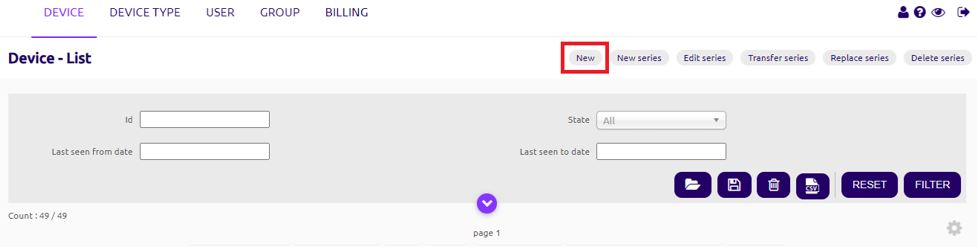
\includegraphics[width=\textwidth]{../../Images/Syde/AddDevice01}
    \captionof{figure}{Sigfox Backend} 
\end{center}


Under Device, click on New.


\begin{center}
    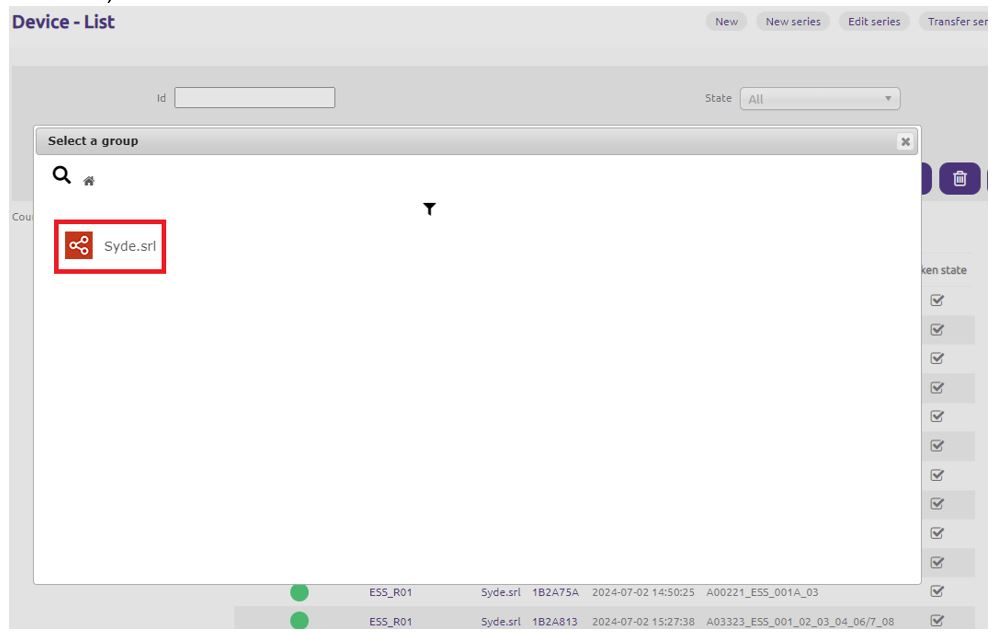
\includegraphics[width=\textwidth]{../../Images/Syde/AddDevice02}
    \captionof{figure}{Sigfox Backend} 
\end{center}

Click on Syde.srl.




\begin{center}
    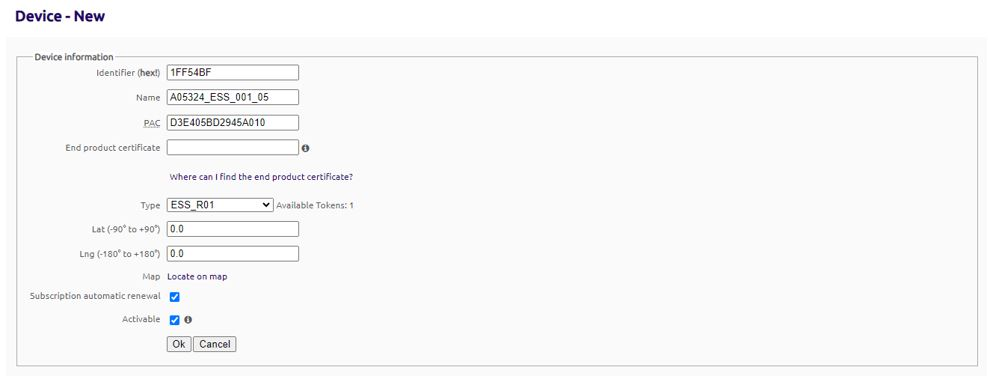
\includegraphics[width=\textwidth]{../../Images/Syde/AddDevice03}
    \captionof{figure}{Sigfox Backend} 
\end{center}

Write the ID, name and PAC, then click on 'Where can i find the end product certificate' and tick the option that appears (prototype sensor).


\begin{center}
    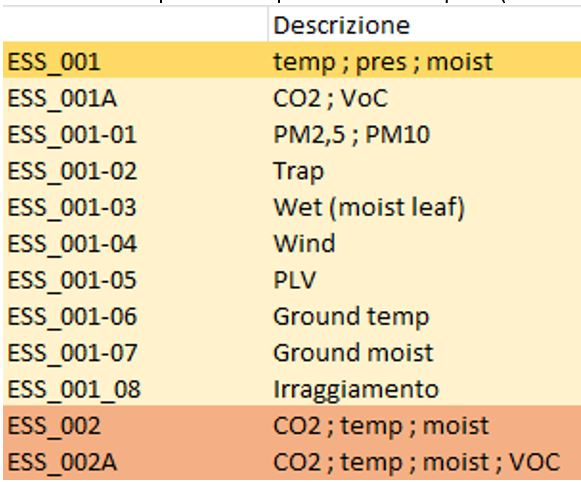
\includegraphics[width=\textwidth]{../../Images/Syde/AddDevice04.JPG}
    \captionof{figure}{legend for sensor name}
 \end{center}

\section{In the case of a sensor with Wi-Fi}

    The whole Sigfox part does not have to be done.
    
    In \FILE{config.json} set 'wifi': true, the wifi name and the password.
    Rename the sensor on the Cloud, writing Device Name (ESS\_...), Device Code (A0...24), Device ID (E465B82..., to be seen with PyCharm) and SigFoxPAC: ----- (no. 5 traits) (for sensor using wifi ONLY).
    

\section{CONSTRUCTION NOTES}
    
    NOTE: Spray clear anti-UV Crystal spray on each blue sensor component.
    
    Screws:
    
\begin{itemize}
    \item ESS Board-Panel HDPE: 3/4 M3x4 screws
    \item  Panel-side blue plugs: 2 screws M4x12 (NOTE: enlarge the holes of the side plugs with a 4.2 mm drill)
    \item  Panel-Board Side: 4/6 M4x25 screws (fit in a cardboard box) (NOTE: enlarge the holes in the base panel with a 4.2 mm drill bit)
    \item USB-C retainer: 2 M3x10 Torse screws
    \item Battery holder: 4 screws M3x16 Torse
    \item Base-High plug: 2 M4x12 screws
    \item []
    \item  Base-White IRR-Panel: 4 screws M4x12 + centre screw M3x10
    \item []
    \item  Base-Template TRAP: 2 screws M3x10 (NOTE: thread the holes)
    \item  Base-Canopy: screw M4x25
    \item  TRAP-Base: screw M3x10 (NOTE: thread the hole)
    \item  Base-Cap painted black: 2 screws M4x12 (NOTE: thread the holes)
    \item  Side plugs: 2 screws M4x30 + screw M3x10 (NOTE: enlarge the holes of the side plugs with the drill with a 4.2 mm drill bit; for the plug with 3 holes, do not enlarge the one isolated at the top on the curved surface)
    \item  Base-white panel: 4 screws M4x12 + centre screw M3x10
    \item  HDPE Base and HDPE Top (PLV): 4 screws M3x40
    \item For the stop of the PLV baseplate: 2 grub screws M4x4
    \item Base-Base-Box Support (PLV): 1 screw M4x30 with nut, 2 screws M4x12
    \item Box-Base Support HDPE: 2 screws M4x12
    \item []
    \item  ANE-Attachment: screw M4x25/30
    \item []
    \item  Panel-Bracket: 2 screws with black head and 1 screw M3x6 Torse (cut) (take care that the latter does not come into contact with the battery)
    
\end{itemize}    
    
\subsection{Nets}

    At the base there are two nets to be fitted, one upper and one lower.
    Cut them out with two special cardboard templates: the rectangular net should be placed at the bottom and should be perforated in the middle for the PLV cables, while the trapezoidal net should be placed at the top and should be perforated in the middle for the ANE cables.
    
\subsection{Battery}

    Tin solder two black crimped leads to the battery cables, then put the sheath around the solder to be shrinked with the heat gun. The cables must then be joined with insulating tape (CAUTION to the order of the cables).
    Glue the battery to the sensor panel with double-sided tape, putting a washer behind the battery to plug the hole.
    
\subsection{Button}

    Put gasket externally between button and panel and internally between button and nut. Put hot glue on the inside.
    
\subsection{Pink cable}

    Put hot glue on the inside.
    
\subsection{BME}

    Wrap silver tape and grey insulation around the BME (keeping the corner with the sensor uncovered) only when reading the temperature through it (does not matter if there is a thermocouple).

It is important to always test the BME to see if it works by deactivating the thermocouple. If the sensor does not read the pressure, then it is a BMEP.

\subsection{Solar panel}

Pay attention to the order of the cables.
Put a dab of hot glue on the cable connection.
Attach to the sensor panel with double-sided tape and silicone.

\subsection{ANE}

The cones must be glued to the rod with liquid Attack.

\subsection{Ground probe}

Put on hot glue to fix it to the sensor box.

\subsection{CO2 (SCD30)}

Sensors with the SCD30 board are indoor and only work when connected to an external power supply (no battery percentage on the app). They also measure temperature and humidity.

\subsection{TVOC}


Transmits every 4 hours (\FILE{config.json} "sgp30time": 3).

\subsection{POW}

Transmits every 4 hours (\FILE{config.json} "dusttime": 3).

\subsection{Sensor packaging}

\begin{itemize}
  \item Make cardboard box with laser cut (large if sensor has ANE and/or PLV, small otherwise)
  \item Put polyethylene foam (white packaging material) in the box
  \item Stick adhesive on front and back of sensor
  \item Switch off sensor
  \item Detach antenna
  \item Put all components into the box (see below)
  \item Tie sensor to carton with green wire
  \item Place the box covering the side sensors on top of the sensor
  \item Write the sensor code [A0(sensor number)(year of construction)] on the box and tick the sensors present
    \item Close the box
    \item Cover the box with white plastic
    \item Attach label indicating the presence of a lithium battery inside
    \item Attach shipping label
\end{itemize}

  Components to be placed in the box
\begin{itemize}
    \item Sensor with USB plug
    \item Antenna
    \item Charging cable
    \item 2 black-headed screws for connection with bracket
    \item Slotted screw and washer for connection with bracket
    \item Bracket
    \item ANE blade (if fitted)
  
\end{itemize}
        